% see http://info.semprag.org/basics for a full description of this template
\documentclass[cm,linguex]{glossa}

% possible options:
% [times] for Times font (default if no option is chosen)
% [cm] for Computer Modern font
% [lucida] for Lucida font (not freely available)
% [brill] open type font, freely downloadable for non-commercial use from http://www.brill.com/about/brill-fonts; requires xetex
% [charis] for CharisSIL font, freely downloadable from http://software.sil.org/charis/
% for the Brill an CharisSIL fonts, you have to use the XeLatex typesetting engine (not pdfLatex)
% for headings, tables, captions, etc., Fira Sans is used: https://www.fontsquirrel.com/fonts/fira-sans
% [biblatex] for using biblatex (the default is natbib, do not load the natbib package in this file, it is loaded automatically via the document class glossa.cls)
% [linguex] loads the linguex example package
% !! a note on the use of linguex: in glossed examples, the third line of the example (the translation) needs to be prefixed with \glt. This is to allow a first line with the name of the language and the source of the example. See example (2) in the text for an illustration.
% !! a note on the use of bibtex: for PhD dissertations to typeset correctly in the references list, the Address field needs to contain the city (for US cities in the format "Santa Cruz, CA")

%\addbibresource{sample.bib}
% the above line is for use with biblatex
% replace this by the name of your bib-file (extension .bib is required)
% comment out if you use natbib/bibtex

\let\B\relax %to resolve a conflict in the definition of these commands between xyling and xunicode (the latter called by fontspec, called by charis)
\let\T\relax
\usepackage{xyling} %for trees; the use of xyling with the CharisSIL font produces poor results in the branches. This problem does not arise with the packages qtree or forest.
\usepackage[linguistics]{forest} %for nice trees!
\usepackage{longtable}

\title[Replication landscape in experimental linguistics]{Assessing the replication landscape in experimental linguistics\\ \bigskip \large Word count: 9520}
% Optional short title inside square brackets, for the running headers.

% \author[Paul \& Vanden Wyngaerd]% short form of the author names for the running header. If no short author is given, no authors print in the headers.
% {%as many authors as you like, each separated by \AND.
%   \spauthor{Waltraud Paul\\
%   \institute{CNRS, CRLAO}\\
%   \small{105, Bd. Raspail, 75005 Paris\\
%   waltraud.paul@ehess.fr}
%   }
%   \AND
%   \spauthor{Guido Vanden Wyngaerd \\
%   \institute{KU Leuven}\\
%   \small{Warmoesberg 26, 1000 Brussel\\
%   guido.vandenwyngaerd@kuleuven.be}
%   }%
% }

\author[Kobrock \& Roettger]{
    \spauthor{Kristina Kobrock\\
  \institute{University of Osnabrück}\\
  \small{\href{mailto:kristina.kobrock@uos.de}{\nolinkurl{kristina.kobrock@uos.de}}}
  }%
  \AND  \spauthor{Timo B. Roettger\\
  \institute{Universitetet i Oslo}\\
  \small{\href{mailto:timo.b.roettger@gmail.com}{\nolinkurl{timo.b.roettger@gmail.com}}}
  }%
  }

\usepackage{natbib}


% tightlist command for lists without linebreak
\providecommand{\tightlist}{%
  \setlength{\itemsep}{0pt}\setlength{\parskip}{0pt}}

% From pandoc table feature
\usepackage{longtable,booktabs,array}
\usepackage{calc} % for calculating minipage widths
% Correct order of tables after \paragraph or \subparagraph
\usepackage{etoolbox}
\makeatletter
\patchcmd\longtable{\par}{\if@noskipsec\mbox{}\fi\par}{}{}
\makeatother
% Allow footnotes in longtable head/foot
\IfFileExists{footnotehyper.sty}{\usepackage{footnotehyper}}{\usepackage{footnote}}
\makesavenoteenv{longtable}




\usepackage{fontspec}
\usepackage{multirow}
\usepackage{multicol}
\usepackage{colortbl}
\usepackage{hhline}
\usepackage{longtable}
\usepackage{array}
\usepackage{hyperref}

\begin{document}


\sffamily
\maketitle

\begin{abstract}
Replications are an integral part of cumulative experimental science. Yet many scientific disciplines do not replicate much because novel confirmatory findings are valued over direct replications. To provide a systematic assessment of the replication landscape in experimental linguistics, the present study estimated replication rates for over 50.000 articles across 98 journals. We used automatic string matching using the Web of Science combined with in-depth manual inspections of 274 papers. The median rate of mentioning the search string ``replicat*'' was as low as 1.7\%. Subsequent manual analyses of articles containing the search string revealed that only 4\% of these contained a direct replication, i.e.~a study that aims to arrive at the same scientific conclusions as an initial study by using exactly the same methodology. Less than half of these direct replications were performed by independent researchers. Thus our data suggest that only 1 in 1250 experimental linguistic articles contains an independent direct replication. We conclude that, similar to neighboring disciplines, experimental linguistics replicates very little, a state of affairs that should be reflected upon.
\end{abstract}

\begin{keywords}
  replication, meta-research, journal impact factor, publishing guidelines
\end{keywords}

\rmfamily

%  Body of the article
\hypertarget{introduction}{%
\section{Introduction}\label{introduction}}

Understanding the inner workings of human language and its cognitive underpinnings has been increasingly shaped by experimental data. With a field that builds its theories on a rapidly growing body of experimental evidence, it is of critical importance to evaluate and substantiate existing findings in the literature because evidence provided by a single study is limited \citep[e.g.,][]{amrhein2019inferential}. Scientists are trained to ensure the reliability and generalizability of scientific findings by conducting direct replication studies, i.e.~studies that aim to arrive at the same scientific conclusions as an initial study by collecting new data and completing new analyses but using the same methodology \citep[see][ for a comprehensive overview of different terminological uses]{barba_terminologies_2018}.

Replications are an integral part of cumulative experimental science \citep[e.g.,][]{campbell_reforms_1969, rosenthal_replication_1990, zwaan_making_2018}. Yet many scientific disciplines do not replicate a lot. Researchers from diverse fields such as psychology \citep{makel_replications_2012}, educational science \citep{makel_facts_2014}, ecology \citep{kelly2019rate}, criminology \citep{mcneeley2015replication}, and economics \citep{mueller2019replication} report on very low numbers of published replications, ranging from 0.02\% in ecology to 2\% in criminology.

One reason for the observed lack of replication studies is the asymmetric incentive system in academia that rewards novel confirmatory findings over direct replications and null results: Replication studies are not very popular because the necessary time and resource investments are not appropriately rewarded \citep[e.g.,][]{koole_rewarding_2012, nosek_scientific_2012}. Both successful replications \citep{madden_how_1995} and repeated failures to replicate \citep[e.g.,][]{doyen_behavioral_2012} are rarely published. Even if they are, replications usually appear in less prestigious outlets than the original findings. These dynamics lead to an abundance of positive findings in the absence of possible conflicting negative evidence \citep[see also][]{fanelli_pressures_2010} and the widely held view that replications lack prestige, originality, or excitement \citep[e.g.,][]{lindsay1993design}.

This perceived lack of prestige additionally comes with the sentiment that direct replications are unnecessary and / or uninformative.
This sentiment expresses itself in two parts: Direct replications are claimed to be theoretically uninformative and conceptual replications are claimed to be sufficient to assess the robustness of a field's empirical foundation \citep[e.g.,][]{stroebe2014alleged, crandall2016scientific}.
However, both of these assumptions are problematic \citep[e.g.,][]{zwaan_making_2018}:
A repeated demonstration that an effect can not be replicated is an important contribution to the field and aids it in calibrating researchers' (un)certainty in the existence of a phenomenon.
Moreover, failed direct replications might uncover important moderators and boundary conditions that explain the discrepancy between an original study and a replication.
Conducting a direct replication operates on the assumption that all critical elements to reproduce the original effect are understood.
If the replication fails, that strong assumption has to be questioned, thus relevant auxiliary hypotheses must be reconsidered, which in turn might weaken the theory.
On the other hand, successful direct replications add important data to the discourse, allowing for more precise estimation of theoretically relevant parameters, and thus help to strengthen the derivation chain between theory and predictions \citep{meehl1990summaries}.

Given these arguments, we consider direct replications theoretically informative and a worthwhile endeavor.
Conceptual replications on the other hand, i.e.~replication attempts that have changed multiple critical design properties of the original study, are often upheld as being more valuable than direct replications because they are assumed to simultaneously address concerns about reliability of an original claim and they are able to extend the original findings.

Conceptual replications are often considered sufficient for a field to move forward under the stipulation that repeated successful conceptual replications will occur only then when the prior research identified a true effect.
However, there is increasing evidence that this strong assumption is empirically not supported.
Without replicating individual studies, biases caused by questionable research practices \citep{john2012measuring}, small sample size \citep{button2013power} and publication bias \citep{fanelli2012negative} can lead to a set of studies that appear to form a coherent empirical foundation of an underlying theory, even if the underlying empirical claims cannot be replicated:
There are now a number of widely studied theories and effects that have been supported by dozens, if not hundreds of conceptual replications, but appear to crumble in light of meta-analyses or systematic direct replication attempts \citep[e.g.,][]{shanks2015romance, wagenmakers2016registered}.
Moreover, conceptual replications can introduce interpretational ambiguity.
A failed conceptual replication can never be considered evidence against the original claim.
It is always possible to attribute a failed conceptual replication to the methodological changes that were made \citep[e.g.,][]{pashler2012replicability}.

In sum, direct replications are an under-appreciated tool to evaluate and cement the empirical and theoretical foundation of a field and must be considered an important complementary tool to conceptual replications.

The observed lack of replication studies across disciplines threatens the very fabric of cumulative progress in experimental science because experimental results are often taken for granted without them ever being replicated which leads to a related problem: If we don't try, we won't fail. The recent past has shown that if we try, we fail more often than we would like to: Coordinated efforts to replicate published findings have uncovered alarmingly low rates of successful replications in fields such as psychology \citep{open_science_collaboration_estimating_2015}, economics \citep{camerer_evaluating_2016}, and social sciences \citep{camerer_evaluating_2018}, a state of affairs that has been referred to as the ``replication crisis'' \citep{fidler_reproducibility_2018}.

The replication crisis is not rooted in a singular cause, but pertains to a network of different practices and incentive structures, all of which conjointly lead to an increase in results that are not replicable. Researchers have identified practices that might have contributed to the wide-spread lack of replicability, including but not limited to too small sample sizes \citep[e.g.,][]{button2013power, vasishth_statistical_2018}, lack of data and materials sharing \citep[e.g.,][]{nosek2015promoting}, use of anti-conservative statistical methods \citep[e.g.,][]{yarkoni2019generalizability}, large analytical flexibility \citep[e.g.,][]{simmons2011false}, and lack of generalizability across diverse contexts and populations \citep{henrich2010weirdest}.

These limitations are present, and maybe even exacerbated in experimental linguistic research: Access to certain linguistic populations is often limited or too cost-intensive, making it difficult to collect sufficiently large samples. Experimental linguistic research is resource-intensive because of equipment cost and complexity, elaborateness of data collection procedures, and computational requirements of data analysis and curation. This often results in studies with small sample sizes and, consequently, with low statistical power \citep[e.g.,][]{casillas2021interlingual, kirby2018mixed}. Statistical analyses in linguistics are often ignoring important assumptions \citep[e.g.,][]{winter2021independence} and are characterized by a large number of researcher degrees of freedom \citep{roettger2019researcher}. Moreover, claims about human language are often based on a small set of languages, limiting their generalizability \citep[e.g.,][]{levisen2019biases, majid2010language}.

In light of the large overlap in research practices between linguistics and neighboring disciplines for which low replication rates and failures of attempts to replicate have been attested, there are raising concerns about both replication rates and replicability in the field of experimental linguistics \citep[e.g.,][]{marsden_replication_2018, roettger_toward_2019, sonning2021replication}. A number of failed replication attempts reported in various subfields of linguistics indicate that these concerns have to be taken seriously \citep[e.g.,][]{chen_chinese_2007, morey2021pre, nieuwland_large-scale_2018, papesh_just_2015, stack_failure_2018, vasishth_statistical_2018, westbury_implicit_2018, jager_interference_2020, nieuwland_anticipating_2020}.

Despite these known problems, there might be only very few published direct replications in linguistics. In their detailed assessment of replications in second language (L2) research, \citet{marsden_replication_2018} explored 67 self-labeled L2 replication studies for a wide variety of characteristics. Their results indicate that for every 400 articles, only one replication study is published which translates into 0.25\% of published studies contain a replication. Following \citet{makel_replications_2012}, we will refer to the proportion of published articles containing at least one replication as the replication rate.
Moreover, the sample of \citet{marsden_replication_2018} did not include a single direct replication study, i.e.~a replication that strictly followed the design of the initial study. This is a state of affairs that is worrisome and warrants further investigation. To our knowledge, there is no systematic assessment of replication rates across experimental linguistics beyond \citet{marsden_replication_2018}. The present paper aims at filling this gap. To gauge the past and current replication landscape in experimental linguistics, track progress over time, and calibrate future policy and training initiatives, it will be useful to assess the prevalence of replications across experimental linguistics and explore their contributing factors.

The present study assesses the frequency of articles containing replications as well as the typology of replication studies that have been published in a representative sample of experimental linguistic journals from 1945 to 2020.
Given the arguments presented above, we are primarily interested in the prevalence of direct replications in the field.
Our study aimed at answering two main questions: ``How many published papers in experimental linguistics contain at least one direct replication?'' and ``Are there factors that affect the replication rates and are they either found at the journal level (e.g.~journal policies, open access, journal impact factor, etc.) or at the study level (e.g.~composition of authors, investigated language, etc.)?''
The study consisted of two analyses:
First, we assessed the frequency of articles mentioning the term replication (search string: replicat*) across 98 linguistic journals.
Second, we manually categorized the type of replication studies (direct, partial, conceptual) in a subset of twenty journals. We then related their replication rates to factors like the years of publication, and the citation counts of both initial and replication study.

\hypertarget{how-often-do-journals-mention-the-term-replicat}{%
\section{How often do journals mention the term replicat*?}\label{how-often-do-journals-mention-the-term-replicat}}

The key dependent variable of the first part of this study was the rate of replication mention for journals relevant to the field of experimental linguistics.

\hypertarget{material-and-methods}{%
\subsection{Material and methods}\label{material-and-methods}}

The study design has been preregistered at 2021-03-08 and can be inspected at \url{https://osf.io/a5xd7/}.

In order to determine the rates of replication mention for individual journals, we drew on a method introduced by \citet{makel_replications_2012}.
First, a sample of 100 journals relevant to the field of experimental linguistics was identified by making use of the search engine \href{https://webofknowledge.com}{``Web of Science'' (https://webofknowledge.com)} (access date: 2021-03-03). We restricted the search results to journals in the web of science category ``Linguistics'' which had at least 100 articles published and a high ratio of articles containing the term experiment* in title, abstract or keywords in order to ensure that the subset contained journals that are relevant for experimental linguistics research. Among those, all articles categorized as having been published in English and between 1945-2020 were taken into account.\footnote{The Web of Science catalog includes articles from 1945 to present. All full available years (at the date of retrieval) have been included in the analysis. The first entries for the category ``Linguistics'' date back to the year 1948 and the first hit for the search term ``replicat*'' was obtained for the year 1969.}

The ratio between overall number of articles and those articles mentioning the term ``experiment*'' ranged between 6.1\% and 60.3\% (with a median of 11.5\%) across journals.
The full sample of journals can be inspected in the appendix of this article.\footnote{Two journals, namely ``Language and Cognitive Processes'' (since 2014: ``Language, Cognition and Neuroscience'') and ``Literary and Linguistic Computing'' (since 2015: ``Digital Scholarship in the Humanities''), have been renamed. The article counts of the old and new journal names were combined under the new name. Our final sample thus included only 98 journals.}

After journal selection, we obtained the total count of articles containing the search term replicat* in title, abstract or keywords for each journal.
Following the method presented by Makel et al. \citeyearpar{makel_replications_2012}, the rates of replication mention were calculated by dividing the number of articles containing the term replicat* by the total number of eligible articles for each journal. As we were only interested in experimental linguistic studies, we only considered articles containing the search term experiment* as eligible.

Rates of replication mention were then related to three journal properties: journal policies with regards to replication studies, journal impact factor and whether the journal publishes open access or not.
To gain an understanding of the journal policies with regards to replication studies, we examined the journals' submission guidelines adopting a method suggested by Martin and Clarke \citeyearpar{martin_are_2017}.
They grouped psychology journals into categories dependent on whether they (explicitly or implicitly) encouraged replication studies or not in their ``instructions to authors'' and ``aims and scope'' sections on the journal websites. For our analysis, we only distinguished between those journals explicitly encouraging replication studies and those that do not.
We extracted journal impact factors via Journal Citation Reports (\url{https://jcr.clarivate.com}).\footnote{The 2019 journal impact factors are calculated by dividing the citations in 2019 to items published in 2017 and 2018 by the total number of citable items in 2017 and 2018.}
We assessed whether journals offered open access publication or not via Web of Science.
We distinguished between three access categories: those journals which are listed in the Directory of Open Access Journals (DOAJ) (``DOAJ gold''), those journals that contained some open access articles (``partial'') and those journals with no option to publish open access (``no'') whatsoever.

We would like to stress that journal-based predictors are not static and obviously change over time. We cannot reliably capture these dynamics. Instead, we snapshot journal policies and impact factors in the year 2019 and use this information as a (rough) proxy for our preregistered objective to relate them to replication rates. As will be discussed below, the model estimates for these predictors are characterized by large amounts of uncertainty, leaving them rather uninformative.

\hypertarget{results-and-discussion}{%
\subsection{Results and Discussion}\label{results-and-discussion}}

Out of the 52302 articles in our sample, 8437 mentioned the term `experiment*' in title, abstract, or keywords and were thus assumed to be articles presenting an experimental investigation.
Out of these articles, 382 contained the term replicat* which results in a mention rate of 4.5\% across experimental linguistic articles.

The distribution of the rate of replication mention substantially varies across journals ranging from 0 to 12.82\%. The median rate of replication mention is 1.7\% (SD = 3.3), a rate that is comparable to what \citet{makel_replications_2012} have reported in their assessment of replications in psychology.
Almost half of all journals (n = 42) did not mention the term in any of their articles.
Figure \ref{fig:topten-plot} illustrates the variation across those journals that exhibited at least one mention of the term.

\begin{figure}

{\centering 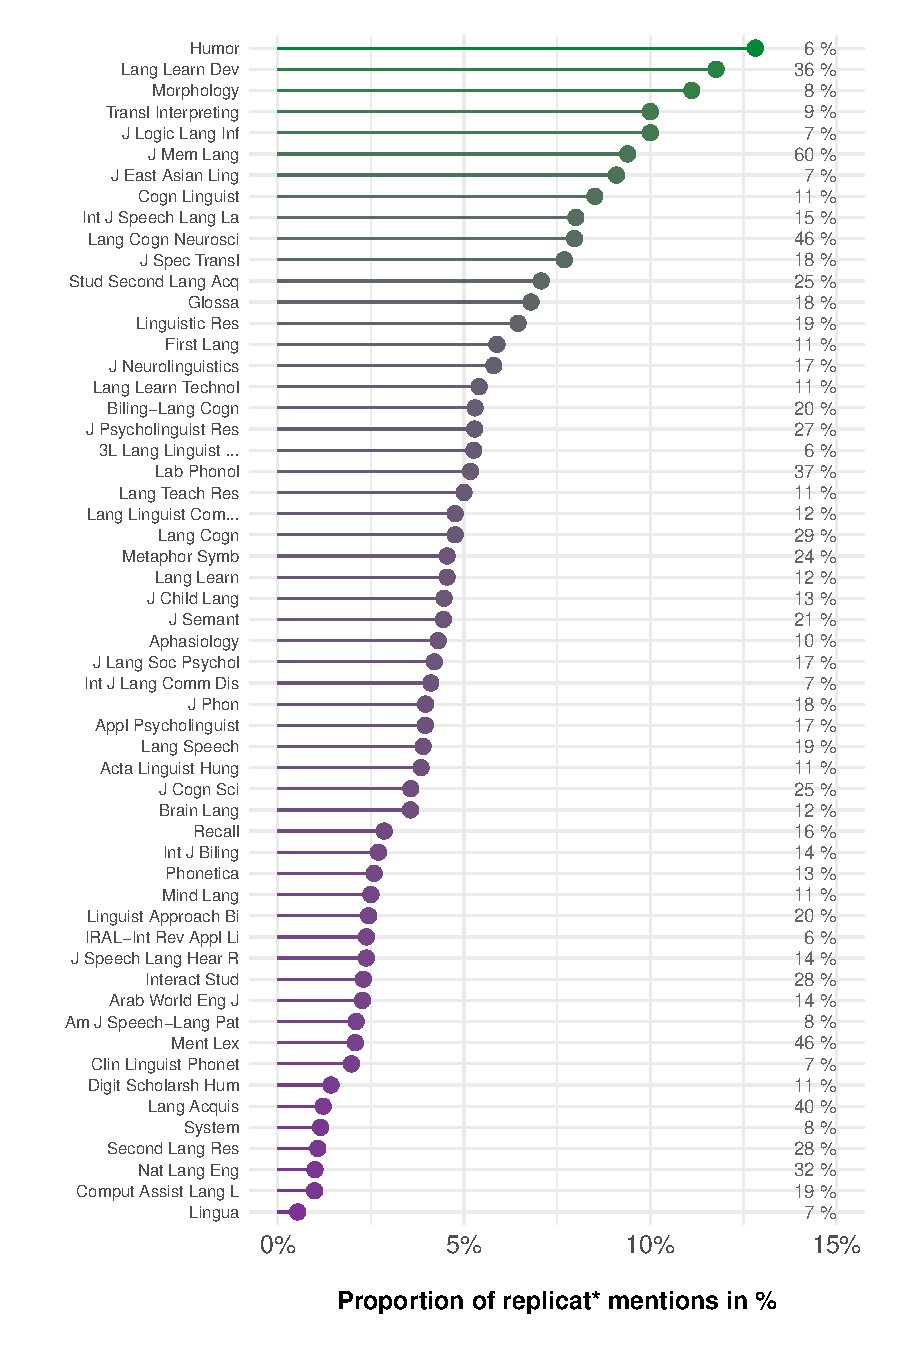
\includegraphics{ReplicationLing_files/figure-latex/topten-plot-1} 

}

\caption{Variation in rate of replicat* mention across those journals that exhibited at least one mention of the term. Numeric values on the right indicate the observed proportion of articles containing the string experiment* in title, abstract or keywords.}\label{fig:topten-plot}
\end{figure}

We statistically estimated the rate of replication mention as predicted relative to the following factors:
centered journal impact factors (continuous, henceforth jif), open access type (no, partial, DOAJ gold), and replication policies (binary: either explicitly encourage or not).\footnote{We diverted from the preregistered protocol after constructive exchanges with our reviewers: We originally planned to use uncentered jif and open access as a binary covariate. Using uncentered jif would have provided an intercept representing journals with a journal impact factor of 0. Centering the variable to the mean jif of our sampled journals allows for a more intuitive interpretation of the coefficients. Second, we preregistered a dichotomization of open access policy which might obscure a more nuanced relationship between open access policy and replication rate. We thus opted for including all three levels of our open access variable in the final model. Both the preregistered and revised models are available in our repository.}
We used Bayesian parameter estimation based on generalized linear regression models with a binomial link function.\footnote{A possible concern of our modelling strategy might be an inflation of zeroes if there are too many journals without a single mention of the search term. A zero-inflated binomial regression can account for such an inflation. Thus, we additionally ran a zero-inflated binomial model. The resulting estimates for our parameters are highly compatible with those from the simpler binomial model. Both models are available in our repository.}
The model was fitted to the proportion of replication mentions per journal using the R package brms \citep{burkner_brms_2016}.
We used weakly informative normal priors centered on 0 (sd = 2.5) for the intercept and Cauchy priors centered on zero (scale = 2.5) for all population-level regression coefficients.
These priors are what is referred to as regularizing \citep{gelman_weakly_2008}, thus making our model conservative with regards to the predictors under investigation.
Four sampling chains with 2000 iterations each have been run for each model, with a warm-up period of 1000 iterations.
For relevant predictor levels and contrasts between predictor levels, we report the posterior probability for the rate of replication mention.
We summarize these distributions by reporting the posterior mean and the 95\% credible intervals (calculated as the highest posterior density interval).

The model estimates the proportion of replication mentions as 3.7\% {[}2.8, 4.7{]} for the average journal impact factor of our sample and the most common open access category ``partial''. The model estimates that the mention rate increases with each integer unit of jif (log odds = 0.36 {[}0.27, 0.46{]}).
Figure \ref{fig:plot-mention-jif} illustrates this relationship.

Further explorations, however, indicate that jif is correlated with the number of experimental studies reported in a journal (Spearman correlation = 0.42).\footnote{This exploratory analysis was not preregistered.}
Given the observed correlation, it remains unclear if the term replicat* is really used more often in high impact journals or simply more common in journals that generally publish more experimental studies (which tend to have higher jifs).

\begin{figure}

{\centering 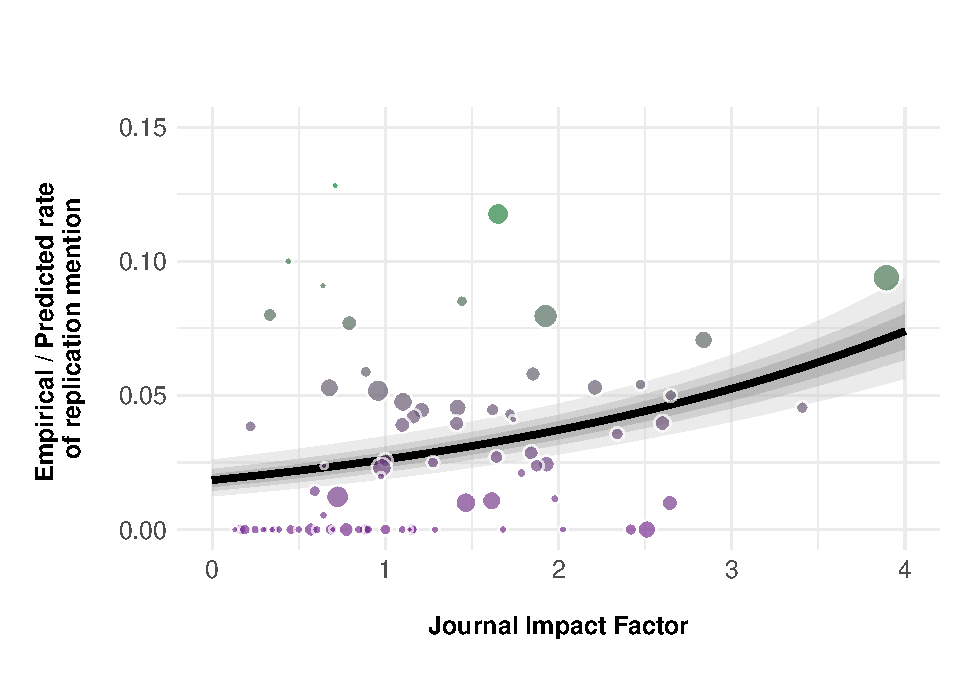
\includegraphics[width=1\linewidth]{ReplicationLing_files/figure-latex/plot-mention-jif-1} 

}

\caption{Estimated and empirical rate of mentioning the term 'replicat*' across sampled journals plotted against their journal impact factor. Each point represents one journal. Point size indicates the proportion of papers categorized as experimental (i.e. larger points indicate journals with more experimental articles). Line and shading indicate model predictions for journals with partial open access and 50/75/95\% credible intervals.}\label{fig:plot-mention-jif}
\end{figure}

The model estimates the impact of whether the journal allows for open access publishing or not and whether replications are explicitly encouraged or not both as positive, i.e.~the term replication is mentioned more often in both open access journals and in journals that explicitly encourage direct replications. Furthermore, the model suggests an ordinal relationship between open access categories and replication mention, characterized by higher rates in DOAJ gold open access journals than in partial open access journals which have higher rates than journals without any open access. However, due to the small number of journals that explicitly encourage direct replications (2 out of 98), and the relatively small number of open access journals (11 out of 98), the uncertainty around all these estimates is substantial (rates increase for DOAJ gold open access: 1.6\% {[}-1.5, 6.1{]}; rates decrease for no open access: -1.9\% {[}-4.4, 7{]}; and rates increase for encouraging replication policies: 0.7\% {[}-1.1, 2.8{]}). We thus won't discuss these results further.

\hypertarget{how-many-articles-containing-the-term-replicat-are-actual-replications}{%
\section{How many articles containing the term replicat* are actual replications?}\label{how-many-articles-containing-the-term-replicat-are-actual-replications}}

The second part of the study had two aims: First, the term replication is commonly used in ambiguous ways, so articles containing the search term were further analyzed to determine whether they indeed reported a replication study or whether they used the term in a different way.
Second, we further investigated what types of replication studies are published and whether replications are becoming more frequent over time. Our target estimand is the proportion of experimental articles containing at least one replication.

\hypertarget{material-and-methods-1}{%
\subsection{Material and methods}\label{material-and-methods-1}}

From the superset of 98 journals obtained above, the 19 journals\footnote{Due to ``Language and Cognitive Processes'' being renamed to ``Language Cognition and Neuroscience'', we did not reach the preregistered target sample of 20.} with the highest proportion of experimental studies were selected for a more detailed analysis while excluding journals for which less than 2 hits (TS=replicat*) could be obtained (see at \url{https://osf.io/f3yp8/} for a list of article counts per journal).
The sampling procedure above resulted in 274 possible self-labeled replication studies with publication years ranging between 1989 and 2020. We included the full set of articles in our sample for manual coding.

We identified whether the article in question indeed presented a replication study or not.
Parts of the papers that were examined were title and abstract of the paper, text before and after occurrences of the search term replicat*, the paragraph before the Methods section as well as the first paragraph of the Discussion section \citep[following and adapting the procedure specified by][]{makel_replication_2016}.
If the authors explicitly claimed that (one of) their research aim(s) was to replicate the result or methods of an initial study, this article was treated as a replication and was submitted to further analysis according to the preregistered coding scheme which can be inspected at \url{https://osf.io/ct2xj/}.

When extracting number and types of changes made to the initial study, we assumed that the authors of a replication study did not make any drastic changes \emph{without} reporting them.
Following Marsden et al. \citeyearpar{marsden_replication_2018}, replication studies were classified according to the number of changes made into three categories: direct replication (0 changes), partial replication (1 change) and conceptual replication (2 or more changes).
We noted the nature of methodological changes as one of the following categories:
experimental paradigm, sample, materials/experimental set-up, dependent variable, independent variable, and control.
Table \ref{tab:coding} shows examples for the five categories that were used for identifying to which of the three types of replications an article belonged.
All of the changes that have been identified by the manual coding procedure are changes that have been reported by the authors of the replication study. Most of these changes have been made by the authors in order to achieve specific goals: Either they aimed at showing that an effect extends to another language, that it is robust across different experimental paradigms or subject groups or how different kinds of measurements, manipulations and controls affect the observed results. As such, we did not consider slight changes in the stimulus materials like the correction of typos but only changes that were identified by the authors as expected to change the results or improve the study in a significant way.
We also recorded the language under investigation.
The information on whether the article was published open access as well as citation counts and years of publication for both studies were obtained from Web of Science.
An author overlap was attested when at least one author was a (co-)author on both studies.
During the coding procedure of the articles, we encountered edge cases that we did not anticipate in our preregistration: When several self-labeled replication studies were mentioned in one article, we chose the first mentioned study for our analysis. If there were one independent, but also one or more inner-paper replications, i.e.~experiments that first replicated an independent initial study and then replicated results from a study in the same article, we selected the independent replication for analysis. Note that since our target estimand is the rate of published articles that contain at least one replication, this choice does not artificially reduce the replication rate.

\providecommand{\docline}[3]{\noalign{\global\setlength{\arrayrulewidth}{#1}}\arrayrulecolor[HTML]{#2}\cline{#3}}

\setlength{\tabcolsep}{2pt}

\renewcommand*{\arraystretch}{1.5}

\begin{longtable}[c]{|p{2.30in}|p{2.30in}}

\caption{Types of changes that determined the type of replication study with examples.
}\label{tab:coding}\\

\hhline{>{\arrayrulecolor[HTML]{666666}\global\arrayrulewidth=2pt}->{\arrayrulecolor[HTML]{666666}\global\arrayrulewidth=2pt}-}

\multicolumn{1}{!{\color[HTML]{000000}\vrule width 0pt}>{\raggedright}p{\dimexpr 2.3in+0\tabcolsep+0\arrayrulewidth}}{\fontsize{11}{11}\selectfont{\textcolor[HTML]{000000}{\global\setmainfont{Arial}{type\ of\ change}}}} & \multicolumn{1}{!{\color[HTML]{000000}\vrule width 0pt}>{\raggedright}p{\dimexpr 2.3in+0\tabcolsep+0\arrayrulewidth}!{\color[HTML]{000000}\vrule width 0pt}}{\fontsize{11}{11}\selectfont{\textcolor[HTML]{000000}{\global\setmainfont{Arial}{examples}}}} \\

\hhline{>{\arrayrulecolor[HTML]{666666}\global\arrayrulewidth=2pt}->{\arrayrulecolor[HTML]{666666}\global\arrayrulewidth=2pt}-}

\endfirsthead

\hhline{>{\arrayrulecolor[HTML]{666666}\global\arrayrulewidth=2pt}->{\arrayrulecolor[HTML]{666666}\global\arrayrulewidth=2pt}-}

\multicolumn{1}{!{\color[HTML]{000000}\vrule width 0pt}>{\raggedright}p{\dimexpr 2.3in+0\tabcolsep+0\arrayrulewidth}}{\fontsize{11}{11}\selectfont{\textcolor[HTML]{000000}{\global\setmainfont{Arial}{type\ of\ change}}}} & \multicolumn{1}{!{\color[HTML]{000000}\vrule width 0pt}>{\raggedright}p{\dimexpr 2.3in+0\tabcolsep+0\arrayrulewidth}!{\color[HTML]{000000}\vrule width 0pt}}{\fontsize{11}{11}\selectfont{\textcolor[HTML]{000000}{\global\setmainfont{Arial}{examples}}}} \\

\hhline{>{\arrayrulecolor[HTML]{666666}\global\arrayrulewidth=2pt}->{\arrayrulecolor[HTML]{666666}\global\arrayrulewidth=2pt}-}\endhead



\multicolumn{1}{!{\color[HTML]{000000}\vrule width 0pt}>{\raggedright}p{\dimexpr 2.3in+0\tabcolsep+0\arrayrulewidth}}{\fontsize{11}{11}\selectfont{\textcolor[HTML]{000000}{\global\setmainfont{Arial}{experimental\ paradigm}}}} & \multicolumn{1}{!{\color[HTML]{000000}\vrule width 0pt}>{\raggedright}p{\dimexpr 2.3in+0\tabcolsep+0\arrayrulewidth}!{\color[HTML]{000000}\vrule width 0pt}}{\fontsize{11}{11}\selectfont{\textcolor[HTML]{000000}{\global\setmainfont{Arial}{explicit\ change\ in\ experimental\ paradigm,\ \linebreak e.g.\ artificial\ grammar\ learning\ paradigm\ →\ oddball\ paradigm}}}} \\





\multicolumn{1}{!{\color[HTML]{000000}\vrule width 0pt}>{\raggedright}p{\dimexpr 2.3in+0\tabcolsep+0\arrayrulewidth}}{\fontsize{11}{11}\selectfont{\textcolor[HTML]{000000}{\global\setmainfont{Arial}{sample}}}} & \multicolumn{1}{!{\color[HTML]{000000}\vrule width 0pt}>{\raggedright}p{\dimexpr 2.3in+0\tabcolsep+0\arrayrulewidth}!{\color[HTML]{000000}\vrule width 0pt}}{\fontsize{11}{11}\selectfont{\textcolor[HTML]{000000}{\global\setmainfont{Arial}{explicit\ change\ in\ population\ under\ investigation\ for\ the\ purpose\ of\ generalizability,\ \linebreak e.g.\ children\ →\ adults,\ \linebreak English\ →\ French,\ \linebreak monolinguals\ →\ bilinguals}}}} \\





\multicolumn{1}{!{\color[HTML]{000000}\vrule width 0pt}>{\raggedright}p{\dimexpr 2.3in+0\tabcolsep+0\arrayrulewidth}}{\fontsize{11}{11}\selectfont{\textcolor[HTML]{000000}{\global\setmainfont{Arial}{materials\ /\ set-up}}}} & \multicolumn{1}{!{\color[HTML]{000000}\vrule width 0pt}>{\raggedright}p{\dimexpr 2.3in+0\tabcolsep+0\arrayrulewidth}!{\color[HTML]{000000}\vrule width 0pt}}{\fontsize{11}{11}\selectfont{\textcolor[HTML]{000000}{\global\setmainfont{Arial}{explicit\ change\ in\ material\ or\ experimental\ set-up,\linebreak e.g.\ change\ in\ materials\ due\ to\ a\ different\ language,\ general\ changes\ to\ the\ stimulus\ material\ or\ presentation\ in\ order\ to\ improve\ the\ study\ (except\ for\ small\ changes\ like\ typos)}}}} \\





\multicolumn{1}{!{\color[HTML]{000000}\vrule width 0pt}>{\raggedright}p{\dimexpr 2.3in+0\tabcolsep+0\arrayrulewidth}}{\fontsize{11}{11}\selectfont{\textcolor[HTML]{000000}{\global\setmainfont{Arial}{dependent\ variable}}}} & \multicolumn{1}{!{\color[HTML]{000000}\vrule width 0pt}>{\raggedright}p{\dimexpr 2.3in+0\tabcolsep+0\arrayrulewidth}!{\color[HTML]{000000}\vrule width 0pt}}{\fontsize{11}{11}\selectfont{\textcolor[HTML]{000000}{\global\setmainfont{Arial}{explicit\ change\ in\ operationalization/measurement\ of\ dependent\ variable(s)\ due\ to\ theory\ change\ or\ a\ different\ measurement\ technique,\ \linebreak e.g.\ response\ times\ →\ ERP\ component}}}} \\





\multicolumn{1}{!{\color[HTML]{000000}\vrule width 0pt}>{\raggedright}p{\dimexpr 2.3in+0\tabcolsep+0\arrayrulewidth}}{\fontsize{11}{11}\selectfont{\textcolor[HTML]{000000}{\global\setmainfont{Arial}{independent\ variable}}}} & \multicolumn{1}{!{\color[HTML]{000000}\vrule width 0pt}>{\raggedright}p{\dimexpr 2.3in+0\tabcolsep+0\arrayrulewidth}!{\color[HTML]{000000}\vrule width 0pt}}{\fontsize{11}{11}\selectfont{\textcolor[HTML]{000000}{\global\setmainfont{Arial}{explicit\ change\ in\ operationalization/measurement\ of\ manipulated\ variable(s),\ \linebreak e.g.\ the\ inclusion\ or\ omission\ of\ specific\ manipulation\ conditions}}}} \\





\multicolumn{1}{!{\color[HTML]{000000}\vrule width 0pt}>{\raggedright}p{\dimexpr 2.3in+0\tabcolsep+0\arrayrulewidth}}{\fontsize{11}{11}\selectfont{\textcolor[HTML]{000000}{\global\setmainfont{Arial}{control}}}} & \multicolumn{1}{!{\color[HTML]{000000}\vrule width 0pt}>{\raggedright}p{\dimexpr 2.3in+0\tabcolsep+0\arrayrulewidth}!{\color[HTML]{000000}\vrule width 0pt}}{\fontsize{11}{11}\selectfont{\textcolor[HTML]{000000}{\global\setmainfont{Arial}{explicit\ change\ in\ control\ variable(s),\ \linebreak e.g.\ adding\ or\ excluding\ a\ specific\ control\ variable}}}} \\

\hhline{>{\arrayrulecolor[HTML]{666666}\global\arrayrulewidth=2pt}->{\arrayrulecolor[HTML]{666666}\global\arrayrulewidth=2pt}-}



\end{longtable}

\hypertarget{results-and-discussion-1}{%
\subsection{Results and Discussion}\label{results-and-discussion-1}}

Out of the 274 articles in the subsample, 262 (95.6\%) indeed presented experimental linguistics research. The remaining 12 (4.4\%) were not experimental in nature, but rather comments, reviews or computational studies. Out of the 262 experimental studies, 151 were self-claimed replications according to our criteria. The remaining 111 mentions were articles that mentioned the term in other contexts or studies that did not specify the concrete aim of replicating an initial study's design or results. Moreover, many papers used the term ``replicated'' in a broad sense that roughly translates into ``finding a similar result'', thus not qualifying as a replication study as defined above.
Out of the replication studies, we categorized 86 (57\%) as conceptual, 56 (37.1\%) as partial, and only 11 (7.3\%) as direct replications.

Looking closer at direct replications, 5 studies were independent studies, i.e.~there was no overlap between authors of the initial study and the replication study.
Out of these independent direct replication studies, 3 were self-labeled as successful replications.
In other words, our sample included only two failed, independent, direct replication attempts. These low rates indicate that replication attempts, and especially direct replication attempts, are rather rare in the experimental linguistics literature - an observation that is in line with replication rates estimated for other research fields \citep{makel_replications_2012, makel_facts_2014, mueller2019replication}.

Figure \ref{fig:stream-plot} illustrates the development of replication studies throughout publication years.
While the overall number of studies increased over the years, the proportion of direct replications remained stable at best.
However, it seems as if there is an increasing number of partial and conceptual replications that was published within the last few years.\footnote{Given the small number of direct replications in our sample, both a descriptive assessment and an inferential assessment as preregistered are very uninformative. The reader is directed to the supplementary materials if they are interested in the model outputs of the preregistered analysis.}
This increase could represent a shift towards replication practices as a direct consequence of renewed attention to the concept of replications caused by the replication crisis.

\begin{figure}

{\centering 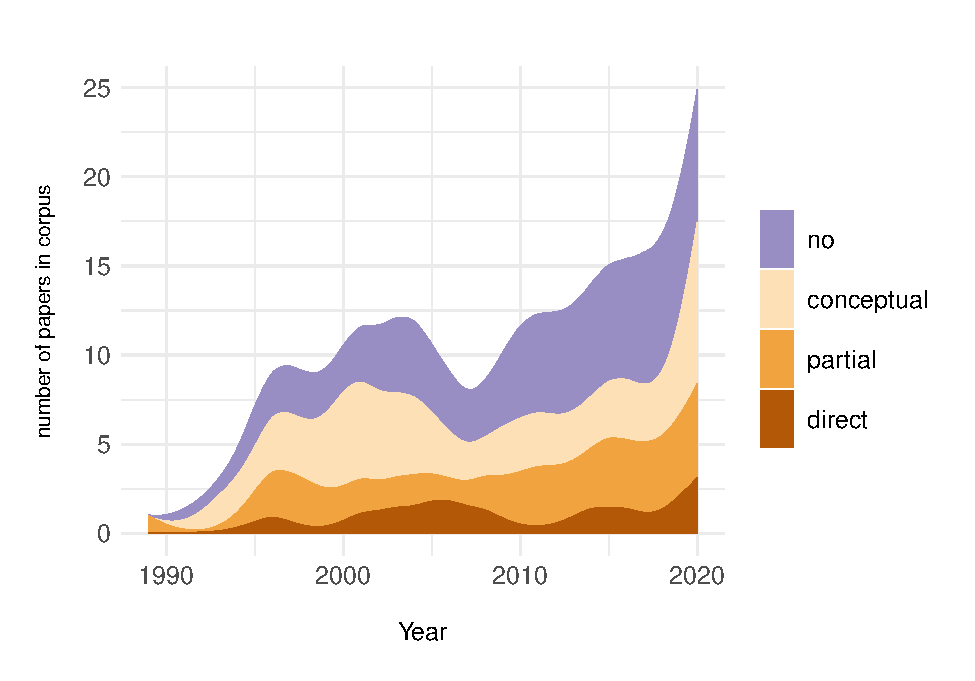
\includegraphics[width=1\linewidth]{ReplicationLing_files/figure-latex/stream-plot-1} 

}

\caption{Development of amount of replication studies published over time. Bandwith of kernel density estimation is set to 0.8.}\label{fig:stream-plot}
\end{figure}

One possible reason for the fact that (direct) replication rates are not increasing for the field according to our analysis could be that experimental linguistics predominantly replicates experimental findings across languages, making the studies by definition only partial/conceptual replications.
However, only 19.9\% of replications targeted a different language than the initial study.
The majority of replication efforts were conducted within the same language as the initial study.
In fact, 67.5\% of all replication studies in our sample had one variety of English as the main language of investigation either in the replication or in the corresponding initial study.

The median number of years between an initial and a replication study is 7 years.
Initial studies were on average 50.1 times cited before a replication was published which corresponds to an average yearly citation rate of 7.2 citations.
This average citation rate is well above the impact factor of core linguistic journals (median journal impact factor in superset: 1.1).
Replication studies were on average only 21 times cited which corresponds to an average yearly citation rate (calculated up to the time of analysis) of 0.5 citations. These results are in line with Marsden et al.'s \citeyearpar{marsden_replication_2018} assessment of second language research. They found that replication studies were on average conducted after more than six years and after over a hundred citations of the original study. They concluded that replications are either only performed or only published after the original study had already substantially impacted the field. Our findings are in line with this interpretation for experimental linguistics.
The observed smaller number of citations of replication studies compared to corresponding initial studies is also in line with the lack of perceived value of replication studies reported in other fields \citep[e.g.,][]{koole_rewarding_2012, nosek_scientific_2012}.

\hypertarget{case-study-of-journal-of-memory-and-language}{%
\subsection{Case study of Journal of Memory and Language}\label{case-study-of-journal-of-memory-and-language}}

The Journal of Memory and Language (JML) accounts for the largest part of articles in our sample (114 out of 274) and is the journal with the highest impact factor (3.9). We conducted a subset analysis of articles published in JML because we were interested in whether our results were affected by this skewed sample.\footnote{Originally, this subset-analysis was planned because in an earlier version of this paper we sampled 50 from the 114 articles published in JML. Following a reviewer's suggestion, we later submitted the full set of JML articles to manual coding. But we keep this analysis to show that our results apply to the whole field and are not mainly influenced by one journal.} We find that 70 (61.9\%) of the 113 experimental JML papers contain replication studies. Of these, 35 (50\%) are conceptual, 30 (42.9\%) are partial, and 5 (7.1\%) are direct replication studies which is in line with the results for the whole sample. Only 3 of the studies published in JML were independent direct replication studies (one of which was successful). We conclude that we have little reason to believe that the large proportion of JML articles in our sample substantially affected our overall results and are confident that our results apply to the field rather than to one journal.

\hypertarget{general-discussion}{%
\section{General discussion}\label{general-discussion}}

The current study aimed at providing a comprehensive survey of published replications in experimental linguistic research.
By analyzing the publication history of over 50000 articles across 98 journals that publish experimental linguistic research, our study found that 4.5\% of experimental linguistic publications used the term replicat* in title, abstract or keywords.
A more thorough analysis of 274 sampled experimental articles containing the term replicat* revealed that only around half of the hits represented actual replication studies, reducing the effective replication rate to 2.5\%. This rate is slightly higher than reports of comparable investigations in psychology \citep[1.6\%,][]{makel_replications_2012}, educational science \citep[0.1\%,][]{makel_facts_2014}, and economics \citep[0.1\%,][]{mueller2019replication}. The higher rate might be due to a methodological choice, however. Due to large plurality of methods in linguistics, we calculated the replication rate based on only those articles that contained the term experiment* (as opposed to all articles in the sample), reducing the denominator substantially.

A closer look at the nature of replication studies revealed that the majority of replication studies were studies that diverted from the initial study by at least one design choice. Only 7.3\% were direct replications, i.e.~studies that directly repeated an initial study without self-reported changes to the design, and only five of these were replications conducted by an independent team of researchers.
Taking together replicat* mention rate and actual replication rate, 0.08\% of experimental studies are independent direct replications in the field of linguistics. In other words, only 1 in 1250 experimental linguistic articles contains an independent direct replication. This clearly indicates that replication attempts, and especially independent direct replication attempts, are still very rare in the experimental linguistics literature.

Before interpreting the results and offering possible ways forward, we need to discuss two important caveats to our study. First, if research articles were not framed as experimental, then they were not included in the analysis. Similarly, if experimental articles were not framed as replications, then they were not categorized as such. These are clear limitations to our search strategy and might lead to an underestimation of the true replication rate. Assuming the false negative rate is not zero, the reported replication rates might change after correction. To circumvent this methodological problem, a large sample of articles would have to undergo manual coding which is not feasible for a large-scale assessment. Future research using alternative assessment methods (possibly machine learning techniques) or more in-depth investigation of either subfields \citep[e.g.,][]{marsden_replication_2018} or specific journals might result in different replication rates.
However, the existence of replication studies that are not referred to as such might also reflect a more general problem: If studies are not framed as replications by using the term replication, readers' ability to connect research to its intellectual precedents is severely limited.

Second, our assessment of replication types relied on two assumptions. On the one hand, we assume that the authors disclosed changes to the initial study in a transparent way. On the other hand, we assume that if changes are disclosed, we were able to extract and interpret these changes accurately. Neither of these assumptions must hold, thus any rates that are generated here are necessarily only a rough proxy of the true replication rate. Nevertheless, given that our findings seem to align well with evidence from other fields as well as an in-depth analysis of a subfield of linguistics \citep{marsden_replication_2018}, we are confident that our conclusion holds.

Although the present study is the first systematic assessment of replication rates in linguistics, our conclusions are hardly surprising. Academic incentive systems do not reward replication studies. Neither journals nor funders encourage them. For example, Martin and Clarke's \citeyearpar{martin_are_2017} survey results suggest that in 2015 only 3\% of psychology journals explicitly state that they will consider publishing replications. Similarly, out of the 98 journals in our sample, only 2 encouraged direct replications. And even if one manages to publish a replication, replication studies are characterized by much lower yearly citation counts compared to corresponding initial studies, leading to a lack of perceived prestige \citep[e.g.,][]{koole_rewarding_2012, nosek_scientific_2012, marsden_replication_2018}. Direct replications simply do not seem worth their costs.

In order to overcome the asymmetry between the cost of direct replication studies and the presently low academic payoff for it, we must re-evaluate the value of direct replications. Funding agencies, journals, but also editors and reviewers, need to start valuing direct replication attempts as much as they value novel findings. For example, we could either dedicate existing journal space to direct replications (e.g.~as its own article type) or create new journals that are specifically dedicated to replication studies.
Journals could help normalizing replication studies by calls for special issues dedicated to replications of influential findings like e.g.~the recent call by the Journal of Memory and Language.\footnote{\url{https://www.journals.elsevier.com/journal-of-memory-and-language/call-for-papers/replicating-influential-findings}}
Another alternative is the Pottery Barn rule, implemented by for example Royal Society Open Science: Once the journal has published a study, it commits to publishing all direct replications of this study.\footnote{ \url{https://royalsociety.org/blog/2018/10/reproducibility-meets-accountability/}}

At the same time, we should attempt to find more resource-efficient ways to both identify replication targets and conduct replication studies. We believe, most people would agree that not every study needs direct replication. Take for example the McGurk effect, i.e.~perceiving a sound that lies in-between an auditory presented component of one sound and a visually presented component of another one \citep{mcgurk1976hearing}. This phenomenon is probably replicated in dozens of linguistic classrooms every semester across the globe.
On the other hand it might be a good idea to evaluate more critically whether a given study is worth replicating. Resources can be saved if studies with poor experimental design, unsuitable measurement approach or inept model specifications are ruled out from direct replication attempts \citep{yarkoni2019generalizability}.
Finding convenient yet effective tools to identify worthwhile replication targets is an active meta-scientific field \citep[e.g.,][]{coles2018costs, isager2021deciding, hardwicke2018bayesian} and feasible algorithms are currently developed and tested \citep{isager2021replication}.
When it comes to more accessible ways to conduct replication studies, several authors have suggested involving our students more rigorously \citep[e.g.,][]{de2019using, frank2012teaching, grahe2012harnessing, roettger_toward_2019}, possibly creating a rich learning experience for our students while at the same time reducing the resource costs of replication studies. Alternatively, resources can be pooled across multi-lab replication efforts, effectively reducing the costs for individual researchers and labs \citep[e.g.,][]{frank2017collaborative, nieuwland_large-scale_2018, open_science_collaboration_estimating_2015}. The StudySwap platform, for example, allows researchers to identify independent labs for conducting a replication attempt of one's study, thus helping researchers to assess the independent replicability of their findings prior to publication \citep{chartier_studyswap_2018}.

We are confident that the field of linguistics can function as a role model for neighboring fields. Although major meta-scientific discourses are held in other fields, linguistics has demonstrated quick uptake of methodological reforms time and time again. A point in case is the swift uptake of Registered Reports\footnote{\url{http://cos.io/rr}}, a new article form in which a study proposal is reviewed before the research is undertaken. While the uptake across disciplines is slow, linguistics has already at least 12 high-impact journal outlets that offer Registered Reports. Moreover, an increasing number of reproducibility initiatives founded in the field during the last few years give hope that the field is continuing to evaluate their past, current, and future practices and successfully face the challenges ahead. This paper was an attempt to contribute to this development. We hope our assessment allows future efforts to track progress over time and calibrate policies across experimental linguistics.

\hypertarget{appendix}{%
\section*{Appendix}\label{appendix}}
\addcontentsline{toc}{section}{Appendix}

\providecommand{\docline}[3]{\noalign{\global\setlength{\arrayrulewidth}{#1}}\arrayrulecolor[HTML]{#2}\cline{#3}}

\setlength{\tabcolsep}{2pt}

\renewcommand*{\arraystretch}{1.5}

\begin{longtable}[c]{|p{1.15in}|p{1.15in}|p{1.15in}|p{1.15in}}

\caption{The full sample of journals sorted by their ratio of experimental linguistics articles.
}\label{tab:journals-sample}\\

\hhline{>{\arrayrulecolor[HTML]{666666}\global\arrayrulewidth=2pt}->{\arrayrulecolor[HTML]{666666}\global\arrayrulewidth=2pt}->{\arrayrulecolor[HTML]{666666}\global\arrayrulewidth=2pt}->{\arrayrulecolor[HTML]{666666}\global\arrayrulewidth=2pt}-}

\multicolumn{1}{!{\color[HTML]{000000}\vrule width 0pt}>{\raggedright}p{\dimexpr 1.15in+0\tabcolsep+0\arrayrulewidth}}{\fontsize{11}{11}\selectfont{\textcolor[HTML]{000000}{\global\setmainfont{Arial}{Journal}}}} & \multicolumn{1}{!{\color[HTML]{000000}\vrule width 0pt}>{\raggedleft}p{\dimexpr 1.15in+0\tabcolsep+0\arrayrulewidth}}{\fontsize{11}{11}\selectfont{\textcolor[HTML]{000000}{\global\setmainfont{Arial}{no.\ articles}}}} & \multicolumn{1}{!{\color[HTML]{000000}\vrule width 0pt}>{\raggedleft}p{\dimexpr 1.15in+0\tabcolsep+0\arrayrulewidth}}{\fontsize{11}{11}\selectfont{\textcolor[HTML]{000000}{\global\setmainfont{Arial}{no.\ exp.\ articles}}}} & \multicolumn{1}{!{\color[HTML]{000000}\vrule width 0pt}>{\raggedleft}p{\dimexpr 1.15in+0\tabcolsep+0\arrayrulewidth}!{\color[HTML]{000000}\vrule width 0pt}}{\fontsize{11}{11}\selectfont{\textcolor[HTML]{000000}{\global\setmainfont{Arial}{ratio\ of\ exp.\ articles\ in\ \%}}}} \\

\hhline{>{\arrayrulecolor[HTML]{666666}\global\arrayrulewidth=2pt}->{\arrayrulecolor[HTML]{666666}\global\arrayrulewidth=2pt}->{\arrayrulecolor[HTML]{666666}\global\arrayrulewidth=2pt}->{\arrayrulecolor[HTML]{666666}\global\arrayrulewidth=2pt}-}

\endfirsthead

\hhline{>{\arrayrulecolor[HTML]{666666}\global\arrayrulewidth=2pt}->{\arrayrulecolor[HTML]{666666}\global\arrayrulewidth=2pt}->{\arrayrulecolor[HTML]{666666}\global\arrayrulewidth=2pt}->{\arrayrulecolor[HTML]{666666}\global\arrayrulewidth=2pt}-}

\multicolumn{1}{!{\color[HTML]{000000}\vrule width 0pt}>{\raggedright}p{\dimexpr 1.15in+0\tabcolsep+0\arrayrulewidth}}{\fontsize{11}{11}\selectfont{\textcolor[HTML]{000000}{\global\setmainfont{Arial}{Journal}}}} & \multicolumn{1}{!{\color[HTML]{000000}\vrule width 0pt}>{\raggedleft}p{\dimexpr 1.15in+0\tabcolsep+0\arrayrulewidth}}{\fontsize{11}{11}\selectfont{\textcolor[HTML]{000000}{\global\setmainfont{Arial}{no.\ articles}}}} & \multicolumn{1}{!{\color[HTML]{000000}\vrule width 0pt}>{\raggedleft}p{\dimexpr 1.15in+0\tabcolsep+0\arrayrulewidth}}{\fontsize{11}{11}\selectfont{\textcolor[HTML]{000000}{\global\setmainfont{Arial}{no.\ exp.\ articles}}}} & \multicolumn{1}{!{\color[HTML]{000000}\vrule width 0pt}>{\raggedleft}p{\dimexpr 1.15in+0\tabcolsep+0\arrayrulewidth}!{\color[HTML]{000000}\vrule width 0pt}}{\fontsize{11}{11}\selectfont{\textcolor[HTML]{000000}{\global\setmainfont{Arial}{ratio\ of\ exp.\ articles\ in\ \%}}}} \\

\hhline{>{\arrayrulecolor[HTML]{666666}\global\arrayrulewidth=2pt}->{\arrayrulecolor[HTML]{666666}\global\arrayrulewidth=2pt}->{\arrayrulecolor[HTML]{666666}\global\arrayrulewidth=2pt}->{\arrayrulecolor[HTML]{666666}\global\arrayrulewidth=2pt}-}\endhead



\multicolumn{1}{!{\color[HTML]{000000}\vrule width 0pt}>{\raggedright}p{\dimexpr 1.15in+0\tabcolsep+0\arrayrulewidth}}{\fontsize{11}{11}\selectfont{\textcolor[HTML]{000000}{\global\setmainfont{Arial}{Journal\ Of\ Memory\ And\ Language}}}} & \multicolumn{1}{!{\color[HTML]{000000}\vrule width 0pt}>{\raggedleft}p{\dimexpr 1.15in+0\tabcolsep+0\arrayrulewidth}}{\fontsize{11}{11}\selectfont{\textcolor[HTML]{000000}{\global\setmainfont{Arial}{2,012}}}} & \multicolumn{1}{!{\color[HTML]{000000}\vrule width 0pt}>{\raggedleft}p{\dimexpr 1.15in+0\tabcolsep+0\arrayrulewidth}}{\fontsize{11}{11}\selectfont{\textcolor[HTML]{000000}{\global\setmainfont{Arial}{1,214}}}} & \multicolumn{1}{!{\color[HTML]{000000}\vrule width 0pt}>{\raggedleft}p{\dimexpr 1.15in+0\tabcolsep+0\arrayrulewidth}!{\color[HTML]{000000}\vrule width 0pt}}{\fontsize{11}{11}\selectfont{\textcolor[HTML]{000000}{\global\setmainfont{Arial}{60.34}}}} \\





\multicolumn{1}{!{\color[HTML]{000000}\vrule width 0pt}>{\raggedright}p{\dimexpr 1.15in+0\tabcolsep+0\arrayrulewidth}}{\fontsize{11}{11}\selectfont{\textcolor[HTML]{000000}{\global\setmainfont{Arial}{Mental\ Lexicon}}}} & \multicolumn{1}{!{\color[HTML]{000000}\vrule width 0pt}>{\raggedleft}p{\dimexpr 1.15in+0\tabcolsep+0\arrayrulewidth}}{\fontsize{11}{11}\selectfont{\textcolor[HTML]{000000}{\global\setmainfont{Arial}{105}}}} & \multicolumn{1}{!{\color[HTML]{000000}\vrule width 0pt}>{\raggedleft}p{\dimexpr 1.15in+0\tabcolsep+0\arrayrulewidth}}{\fontsize{11}{11}\selectfont{\textcolor[HTML]{000000}{\global\setmainfont{Arial}{48}}}} & \multicolumn{1}{!{\color[HTML]{000000}\vrule width 0pt}>{\raggedleft}p{\dimexpr 1.15in+0\tabcolsep+0\arrayrulewidth}!{\color[HTML]{000000}\vrule width 0pt}}{\fontsize{11}{11}\selectfont{\textcolor[HTML]{000000}{\global\setmainfont{Arial}{45.71}}}} \\





\multicolumn{1}{!{\color[HTML]{000000}\vrule width 0pt}>{\raggedright}p{\dimexpr 1.15in+0\tabcolsep+0\arrayrulewidth}}{\fontsize{11}{11}\selectfont{\textcolor[HTML]{000000}{\global\setmainfont{Arial}{Language\ Acquisition}}}} & \multicolumn{1}{!{\color[HTML]{000000}\vrule width 0pt}>{\raggedleft}p{\dimexpr 1.15in+0\tabcolsep+0\arrayrulewidth}}{\fontsize{11}{11}\selectfont{\textcolor[HTML]{000000}{\global\setmainfont{Arial}{207}}}} & \multicolumn{1}{!{\color[HTML]{000000}\vrule width 0pt}>{\raggedleft}p{\dimexpr 1.15in+0\tabcolsep+0\arrayrulewidth}}{\fontsize{11}{11}\selectfont{\textcolor[HTML]{000000}{\global\setmainfont{Arial}{82}}}} & \multicolumn{1}{!{\color[HTML]{000000}\vrule width 0pt}>{\raggedleft}p{\dimexpr 1.15in+0\tabcolsep+0\arrayrulewidth}!{\color[HTML]{000000}\vrule width 0pt}}{\fontsize{11}{11}\selectfont{\textcolor[HTML]{000000}{\global\setmainfont{Arial}{39.61}}}} \\





\multicolumn{1}{!{\color[HTML]{000000}\vrule width 0pt}>{\raggedright}p{\dimexpr 1.15in+0\tabcolsep+0\arrayrulewidth}}{\fontsize{11}{11}\selectfont{\textcolor[HTML]{000000}{\global\setmainfont{Arial}{Language\ Cognition\ And\ Neuroscience}}}} & \multicolumn{1}{!{\color[HTML]{000000}\vrule width 0pt}>{\raggedleft}p{\dimexpr 1.15in+0\tabcolsep+0\arrayrulewidth}}{\fontsize{11}{11}\selectfont{\textcolor[HTML]{000000}{\global\setmainfont{Arial}{1,373}}}} & \multicolumn{1}{!{\color[HTML]{000000}\vrule width 0pt}>{\raggedleft}p{\dimexpr 1.15in+0\tabcolsep+0\arrayrulewidth}}{\fontsize{11}{11}\selectfont{\textcolor[HTML]{000000}{\global\setmainfont{Arial}{628}}}} & \multicolumn{1}{!{\color[HTML]{000000}\vrule width 0pt}>{\raggedleft}p{\dimexpr 1.15in+0\tabcolsep+0\arrayrulewidth}!{\color[HTML]{000000}\vrule width 0pt}}{\fontsize{11}{11}\selectfont{\textcolor[HTML]{000000}{\global\setmainfont{Arial}{45.74}}}} \\





\multicolumn{1}{!{\color[HTML]{000000}\vrule width 0pt}>{\raggedright}p{\dimexpr 1.15in+0\tabcolsep+0\arrayrulewidth}}{\fontsize{11}{11}\selectfont{\textcolor[HTML]{000000}{\global\setmainfont{Arial}{Laboratory\ Phonology}}}} & \multicolumn{1}{!{\color[HTML]{000000}\vrule width 0pt}>{\raggedleft}p{\dimexpr 1.15in+0\tabcolsep+0\arrayrulewidth}}{\fontsize{11}{11}\selectfont{\textcolor[HTML]{000000}{\global\setmainfont{Arial}{155}}}} & \multicolumn{1}{!{\color[HTML]{000000}\vrule width 0pt}>{\raggedleft}p{\dimexpr 1.15in+0\tabcolsep+0\arrayrulewidth}}{\fontsize{11}{11}\selectfont{\textcolor[HTML]{000000}{\global\setmainfont{Arial}{58}}}} & \multicolumn{1}{!{\color[HTML]{000000}\vrule width 0pt}>{\raggedleft}p{\dimexpr 1.15in+0\tabcolsep+0\arrayrulewidth}!{\color[HTML]{000000}\vrule width 0pt}}{\fontsize{11}{11}\selectfont{\textcolor[HTML]{000000}{\global\setmainfont{Arial}{37.42}}}} \\





\multicolumn{1}{!{\color[HTML]{000000}\vrule width 0pt}>{\raggedright}p{\dimexpr 1.15in+0\tabcolsep+0\arrayrulewidth}}{\fontsize{11}{11}\selectfont{\textcolor[HTML]{000000}{\global\setmainfont{Arial}{Language\ Learning\ And\ Development}}}} & \multicolumn{1}{!{\color[HTML]{000000}\vrule width 0pt}>{\raggedleft}p{\dimexpr 1.15in+0\tabcolsep+0\arrayrulewidth}}{\fontsize{11}{11}\selectfont{\textcolor[HTML]{000000}{\global\setmainfont{Arial}{141}}}} & \multicolumn{1}{!{\color[HTML]{000000}\vrule width 0pt}>{\raggedleft}p{\dimexpr 1.15in+0\tabcolsep+0\arrayrulewidth}}{\fontsize{11}{11}\selectfont{\textcolor[HTML]{000000}{\global\setmainfont{Arial}{51}}}} & \multicolumn{1}{!{\color[HTML]{000000}\vrule width 0pt}>{\raggedleft}p{\dimexpr 1.15in+0\tabcolsep+0\arrayrulewidth}!{\color[HTML]{000000}\vrule width 0pt}}{\fontsize{11}{11}\selectfont{\textcolor[HTML]{000000}{\global\setmainfont{Arial}{36.17}}}} \\





\multicolumn{1}{!{\color[HTML]{000000}\vrule width 0pt}>{\raggedright}p{\dimexpr 1.15in+0\tabcolsep+0\arrayrulewidth}}{\fontsize{11}{11}\selectfont{\textcolor[HTML]{000000}{\global\setmainfont{Arial}{Natural\ Language\ Engineering}}}} & \multicolumn{1}{!{\color[HTML]{000000}\vrule width 0pt}>{\raggedleft}p{\dimexpr 1.15in+0\tabcolsep+0\arrayrulewidth}}{\fontsize{11}{11}\selectfont{\textcolor[HTML]{000000}{\global\setmainfont{Arial}{312}}}} & \multicolumn{1}{!{\color[HTML]{000000}\vrule width 0pt}>{\raggedleft}p{\dimexpr 1.15in+0\tabcolsep+0\arrayrulewidth}}{\fontsize{11}{11}\selectfont{\textcolor[HTML]{000000}{\global\setmainfont{Arial}{100}}}} & \multicolumn{1}{!{\color[HTML]{000000}\vrule width 0pt}>{\raggedleft}p{\dimexpr 1.15in+0\tabcolsep+0\arrayrulewidth}!{\color[HTML]{000000}\vrule width 0pt}}{\fontsize{11}{11}\selectfont{\textcolor[HTML]{000000}{\global\setmainfont{Arial}{32.05}}}} \\





\multicolumn{1}{!{\color[HTML]{000000}\vrule width 0pt}>{\raggedright}p{\dimexpr 1.15in+0\tabcolsep+0\arrayrulewidth}}{\fontsize{11}{11}\selectfont{\textcolor[HTML]{000000}{\global\setmainfont{Arial}{Lecture\ Notes\ In\ Computer\ Science}}}} & \multicolumn{1}{!{\color[HTML]{000000}\vrule width 0pt}>{\raggedleft}p{\dimexpr 1.15in+0\tabcolsep+0\arrayrulewidth}}{\fontsize{11}{11}\selectfont{\textcolor[HTML]{000000}{\global\setmainfont{Arial}{150}}}} & \multicolumn{1}{!{\color[HTML]{000000}\vrule width 0pt}>{\raggedleft}p{\dimexpr 1.15in+0\tabcolsep+0\arrayrulewidth}}{\fontsize{11}{11}\selectfont{\textcolor[HTML]{000000}{\global\setmainfont{Arial}{46}}}} & \multicolumn{1}{!{\color[HTML]{000000}\vrule width 0pt}>{\raggedleft}p{\dimexpr 1.15in+0\tabcolsep+0\arrayrulewidth}!{\color[HTML]{000000}\vrule width 0pt}}{\fontsize{11}{11}\selectfont{\textcolor[HTML]{000000}{\global\setmainfont{Arial}{30.67}}}} \\





\multicolumn{1}{!{\color[HTML]{000000}\vrule width 0pt}>{\raggedright}p{\dimexpr 1.15in+0\tabcolsep+0\arrayrulewidth}}{\fontsize{11}{11}\selectfont{\textcolor[HTML]{000000}{\global\setmainfont{Arial}{Language\ And\ Cognition}}}} & \multicolumn{1}{!{\color[HTML]{000000}\vrule width 0pt}>{\raggedleft}p{\dimexpr 1.15in+0\tabcolsep+0\arrayrulewidth}}{\fontsize{11}{11}\selectfont{\textcolor[HTML]{000000}{\global\setmainfont{Arial}{144}}}} & \multicolumn{1}{!{\color[HTML]{000000}\vrule width 0pt}>{\raggedleft}p{\dimexpr 1.15in+0\tabcolsep+0\arrayrulewidth}}{\fontsize{11}{11}\selectfont{\textcolor[HTML]{000000}{\global\setmainfont{Arial}{42}}}} & \multicolumn{1}{!{\color[HTML]{000000}\vrule width 0pt}>{\raggedleft}p{\dimexpr 1.15in+0\tabcolsep+0\arrayrulewidth}!{\color[HTML]{000000}\vrule width 0pt}}{\fontsize{11}{11}\selectfont{\textcolor[HTML]{000000}{\global\setmainfont{Arial}{29.17}}}} \\





\multicolumn{1}{!{\color[HTML]{000000}\vrule width 0pt}>{\raggedright}p{\dimexpr 1.15in+0\tabcolsep+0\arrayrulewidth}}{\fontsize{11}{11}\selectfont{\textcolor[HTML]{000000}{\global\setmainfont{Arial}{Interaction\ Studies}}}} & \multicolumn{1}{!{\color[HTML]{000000}\vrule width 0pt}>{\raggedleft}p{\dimexpr 1.15in+0\tabcolsep+0\arrayrulewidth}}{\fontsize{11}{11}\selectfont{\textcolor[HTML]{000000}{\global\setmainfont{Arial}{312}}}} & \multicolumn{1}{!{\color[HTML]{000000}\vrule width 0pt}>{\raggedleft}p{\dimexpr 1.15in+0\tabcolsep+0\arrayrulewidth}}{\fontsize{11}{11}\selectfont{\textcolor[HTML]{000000}{\global\setmainfont{Arial}{87}}}} & \multicolumn{1}{!{\color[HTML]{000000}\vrule width 0pt}>{\raggedleft}p{\dimexpr 1.15in+0\tabcolsep+0\arrayrulewidth}!{\color[HTML]{000000}\vrule width 0pt}}{\fontsize{11}{11}\selectfont{\textcolor[HTML]{000000}{\global\setmainfont{Arial}{27.88}}}} \\





\multicolumn{1}{!{\color[HTML]{000000}\vrule width 0pt}>{\raggedright}p{\dimexpr 1.15in+0\tabcolsep+0\arrayrulewidth}}{\fontsize{11}{11}\selectfont{\textcolor[HTML]{000000}{\global\setmainfont{Arial}{Second\ Language\ Research}}}} & \multicolumn{1}{!{\color[HTML]{000000}\vrule width 0pt}>{\raggedleft}p{\dimexpr 1.15in+0\tabcolsep+0\arrayrulewidth}}{\fontsize{11}{11}\selectfont{\textcolor[HTML]{000000}{\global\setmainfont{Arial}{338}}}} & \multicolumn{1}{!{\color[HTML]{000000}\vrule width 0pt}>{\raggedleft}p{\dimexpr 1.15in+0\tabcolsep+0\arrayrulewidth}}{\fontsize{11}{11}\selectfont{\textcolor[HTML]{000000}{\global\setmainfont{Arial}{93}}}} & \multicolumn{1}{!{\color[HTML]{000000}\vrule width 0pt}>{\raggedleft}p{\dimexpr 1.15in+0\tabcolsep+0\arrayrulewidth}!{\color[HTML]{000000}\vrule width 0pt}}{\fontsize{11}{11}\selectfont{\textcolor[HTML]{000000}{\global\setmainfont{Arial}{27.51}}}} \\





\multicolumn{1}{!{\color[HTML]{000000}\vrule width 0pt}>{\raggedright}p{\dimexpr 1.15in+0\tabcolsep+0\arrayrulewidth}}{\fontsize{11}{11}\selectfont{\textcolor[HTML]{000000}{\global\setmainfont{Arial}{Journal\ Of\ Psycholinguistic\ Research}}}} & \multicolumn{1}{!{\color[HTML]{000000}\vrule width 0pt}>{\raggedleft}p{\dimexpr 1.15in+0\tabcolsep+0\arrayrulewidth}}{\fontsize{11}{11}\selectfont{\textcolor[HTML]{000000}{\global\setmainfont{Arial}{1,691}}}} & \multicolumn{1}{!{\color[HTML]{000000}\vrule width 0pt}>{\raggedleft}p{\dimexpr 1.15in+0\tabcolsep+0\arrayrulewidth}}{\fontsize{11}{11}\selectfont{\textcolor[HTML]{000000}{\global\setmainfont{Arial}{454}}}} & \multicolumn{1}{!{\color[HTML]{000000}\vrule width 0pt}>{\raggedleft}p{\dimexpr 1.15in+0\tabcolsep+0\arrayrulewidth}!{\color[HTML]{000000}\vrule width 0pt}}{\fontsize{11}{11}\selectfont{\textcolor[HTML]{000000}{\global\setmainfont{Arial}{26.85}}}} \\





\multicolumn{1}{!{\color[HTML]{000000}\vrule width 0pt}>{\raggedright}p{\dimexpr 1.15in+0\tabcolsep+0\arrayrulewidth}}{\fontsize{11}{11}\selectfont{\textcolor[HTML]{000000}{\global\setmainfont{Arial}{Studies\ In\ Second\ Language\ Acquisition}}}} & \multicolumn{1}{!{\color[HTML]{000000}\vrule width 0pt}>{\raggedleft}p{\dimexpr 1.15in+0\tabcolsep+0\arrayrulewidth}}{\fontsize{11}{11}\selectfont{\textcolor[HTML]{000000}{\global\setmainfont{Arial}{389}}}} & \multicolumn{1}{!{\color[HTML]{000000}\vrule width 0pt}>{\raggedleft}p{\dimexpr 1.15in+0\tabcolsep+0\arrayrulewidth}}{\fontsize{11}{11}\selectfont{\textcolor[HTML]{000000}{\global\setmainfont{Arial}{99}}}} & \multicolumn{1}{!{\color[HTML]{000000}\vrule width 0pt}>{\raggedleft}p{\dimexpr 1.15in+0\tabcolsep+0\arrayrulewidth}!{\color[HTML]{000000}\vrule width 0pt}}{\fontsize{11}{11}\selectfont{\textcolor[HTML]{000000}{\global\setmainfont{Arial}{25.45}}}} \\





\multicolumn{1}{!{\color[HTML]{000000}\vrule width 0pt}>{\raggedright}p{\dimexpr 1.15in+0\tabcolsep+0\arrayrulewidth}}{\fontsize{11}{11}\selectfont{\textcolor[HTML]{000000}{\global\setmainfont{Arial}{Computational\ Linguistics}}}} & \multicolumn{1}{!{\color[HTML]{000000}\vrule width 0pt}>{\raggedleft}p{\dimexpr 1.15in+0\tabcolsep+0\arrayrulewidth}}{\fontsize{11}{11}\selectfont{\textcolor[HTML]{000000}{\global\setmainfont{Arial}{521}}}} & \multicolumn{1}{!{\color[HTML]{000000}\vrule width 0pt}>{\raggedleft}p{\dimexpr 1.15in+0\tabcolsep+0\arrayrulewidth}}{\fontsize{11}{11}\selectfont{\textcolor[HTML]{000000}{\global\setmainfont{Arial}{130}}}} & \multicolumn{1}{!{\color[HTML]{000000}\vrule width 0pt}>{\raggedleft}p{\dimexpr 1.15in+0\tabcolsep+0\arrayrulewidth}!{\color[HTML]{000000}\vrule width 0pt}}{\fontsize{11}{11}\selectfont{\textcolor[HTML]{000000}{\global\setmainfont{Arial}{24.95}}}} \\





\multicolumn{1}{!{\color[HTML]{000000}\vrule width 0pt}>{\raggedright}p{\dimexpr 1.15in+0\tabcolsep+0\arrayrulewidth}}{\fontsize{11}{11}\selectfont{\textcolor[HTML]{000000}{\global\setmainfont{Arial}{Journal\ Of\ Cognitive\ Science}}}} & \multicolumn{1}{!{\color[HTML]{000000}\vrule width 0pt}>{\raggedleft}p{\dimexpr 1.15in+0\tabcolsep+0\arrayrulewidth}}{\fontsize{11}{11}\selectfont{\textcolor[HTML]{000000}{\global\setmainfont{Arial}{114}}}} & \multicolumn{1}{!{\color[HTML]{000000}\vrule width 0pt}>{\raggedleft}p{\dimexpr 1.15in+0\tabcolsep+0\arrayrulewidth}}{\fontsize{11}{11}\selectfont{\textcolor[HTML]{000000}{\global\setmainfont{Arial}{28}}}} & \multicolumn{1}{!{\color[HTML]{000000}\vrule width 0pt}>{\raggedleft}p{\dimexpr 1.15in+0\tabcolsep+0\arrayrulewidth}!{\color[HTML]{000000}\vrule width 0pt}}{\fontsize{11}{11}\selectfont{\textcolor[HTML]{000000}{\global\setmainfont{Arial}{24.56}}}} \\





\multicolumn{1}{!{\color[HTML]{000000}\vrule width 0pt}>{\raggedright}p{\dimexpr 1.15in+0\tabcolsep+0\arrayrulewidth}}{\fontsize{11}{11}\selectfont{\textcolor[HTML]{000000}{\global\setmainfont{Arial}{Metaphor\ And\ Symbol}}}} & \multicolumn{1}{!{\color[HTML]{000000}\vrule width 0pt}>{\raggedleft}p{\dimexpr 1.15in+0\tabcolsep+0\arrayrulewidth}}{\fontsize{11}{11}\selectfont{\textcolor[HTML]{000000}{\global\setmainfont{Arial}{278}}}} & \multicolumn{1}{!{\color[HTML]{000000}\vrule width 0pt}>{\raggedleft}p{\dimexpr 1.15in+0\tabcolsep+0\arrayrulewidth}}{\fontsize{11}{11}\selectfont{\textcolor[HTML]{000000}{\global\setmainfont{Arial}{66}}}} & \multicolumn{1}{!{\color[HTML]{000000}\vrule width 0pt}>{\raggedleft}p{\dimexpr 1.15in+0\tabcolsep+0\arrayrulewidth}!{\color[HTML]{000000}\vrule width 0pt}}{\fontsize{11}{11}\selectfont{\textcolor[HTML]{000000}{\global\setmainfont{Arial}{23.74}}}} \\





\multicolumn{1}{!{\color[HTML]{000000}\vrule width 0pt}>{\raggedright}p{\dimexpr 1.15in+0\tabcolsep+0\arrayrulewidth}}{\fontsize{11}{11}\selectfont{\textcolor[HTML]{000000}{\global\setmainfont{Arial}{Lecture\ Notes\ In\ Artificial\ Intelligence}}}} & \multicolumn{1}{!{\color[HTML]{000000}\vrule width 0pt}>{\raggedleft}p{\dimexpr 1.15in+0\tabcolsep+0\arrayrulewidth}}{\fontsize{11}{11}\selectfont{\textcolor[HTML]{000000}{\global\setmainfont{Arial}{113}}}} & \multicolumn{1}{!{\color[HTML]{000000}\vrule width 0pt}>{\raggedleft}p{\dimexpr 1.15in+0\tabcolsep+0\arrayrulewidth}}{\fontsize{11}{11}\selectfont{\textcolor[HTML]{000000}{\global\setmainfont{Arial}{26}}}} & \multicolumn{1}{!{\color[HTML]{000000}\vrule width 0pt}>{\raggedleft}p{\dimexpr 1.15in+0\tabcolsep+0\arrayrulewidth}!{\color[HTML]{000000}\vrule width 0pt}}{\fontsize{11}{11}\selectfont{\textcolor[HTML]{000000}{\global\setmainfont{Arial}{23.01}}}} \\





\multicolumn{1}{!{\color[HTML]{000000}\vrule width 0pt}>{\raggedright}p{\dimexpr 1.15in+0\tabcolsep+0\arrayrulewidth}}{\fontsize{11}{11}\selectfont{\textcolor[HTML]{000000}{\global\setmainfont{Arial}{Journal\ Of\ Semantics}}}} & \multicolumn{1}{!{\color[HTML]{000000}\vrule width 0pt}>{\raggedleft}p{\dimexpr 1.15in+0\tabcolsep+0\arrayrulewidth}}{\fontsize{11}{11}\selectfont{\textcolor[HTML]{000000}{\global\setmainfont{Arial}{218}}}} & \multicolumn{1}{!{\color[HTML]{000000}\vrule width 0pt}>{\raggedleft}p{\dimexpr 1.15in+0\tabcolsep+0\arrayrulewidth}}{\fontsize{11}{11}\selectfont{\textcolor[HTML]{000000}{\global\setmainfont{Arial}{45}}}} & \multicolumn{1}{!{\color[HTML]{000000}\vrule width 0pt}>{\raggedleft}p{\dimexpr 1.15in+0\tabcolsep+0\arrayrulewidth}!{\color[HTML]{000000}\vrule width 0pt}}{\fontsize{11}{11}\selectfont{\textcolor[HTML]{000000}{\global\setmainfont{Arial}{20.64}}}} \\





\multicolumn{1}{!{\color[HTML]{000000}\vrule width 0pt}>{\raggedright}p{\dimexpr 1.15in+0\tabcolsep+0\arrayrulewidth}}{\fontsize{11}{11}\selectfont{\textcolor[HTML]{000000}{\global\setmainfont{Arial}{Linguistic\ Approaches\ To\ Bilingualism}}}} & \multicolumn{1}{!{\color[HTML]{000000}\vrule width 0pt}>{\raggedleft}p{\dimexpr 1.15in+0\tabcolsep+0\arrayrulewidth}}{\fontsize{11}{11}\selectfont{\textcolor[HTML]{000000}{\global\setmainfont{Arial}{204}}}} & \multicolumn{1}{!{\color[HTML]{000000}\vrule width 0pt}>{\raggedleft}p{\dimexpr 1.15in+0\tabcolsep+0\arrayrulewidth}}{\fontsize{11}{11}\selectfont{\textcolor[HTML]{000000}{\global\setmainfont{Arial}{41}}}} & \multicolumn{1}{!{\color[HTML]{000000}\vrule width 0pt}>{\raggedleft}p{\dimexpr 1.15in+0\tabcolsep+0\arrayrulewidth}!{\color[HTML]{000000}\vrule width 0pt}}{\fontsize{11}{11}\selectfont{\textcolor[HTML]{000000}{\global\setmainfont{Arial}{20.10}}}} \\





\multicolumn{1}{!{\color[HTML]{000000}\vrule width 0pt}>{\raggedright}p{\dimexpr 1.15in+0\tabcolsep+0\arrayrulewidth}}{\fontsize{11}{11}\selectfont{\textcolor[HTML]{000000}{\global\setmainfont{Arial}{Bilingualism\ Language\ And\ Cognition}}}} & \multicolumn{1}{!{\color[HTML]{000000}\vrule width 0pt}>{\raggedleft}p{\dimexpr 1.15in+0\tabcolsep+0\arrayrulewidth}}{\fontsize{11}{11}\selectfont{\textcolor[HTML]{000000}{\global\setmainfont{Arial}{753}}}} & \multicolumn{1}{!{\color[HTML]{000000}\vrule width 0pt}>{\raggedleft}p{\dimexpr 1.15in+0\tabcolsep+0\arrayrulewidth}}{\fontsize{11}{11}\selectfont{\textcolor[HTML]{000000}{\global\setmainfont{Arial}{151}}}} & \multicolumn{1}{!{\color[HTML]{000000}\vrule width 0pt}>{\raggedleft}p{\dimexpr 1.15in+0\tabcolsep+0\arrayrulewidth}!{\color[HTML]{000000}\vrule width 0pt}}{\fontsize{11}{11}\selectfont{\textcolor[HTML]{000000}{\global\setmainfont{Arial}{20.05}}}} \\





\multicolumn{1}{!{\color[HTML]{000000}\vrule width 0pt}>{\raggedright}p{\dimexpr 1.15in+0\tabcolsep+0\arrayrulewidth}}{\fontsize{11}{11}\selectfont{\textcolor[HTML]{000000}{\global\setmainfont{Arial}{Computer\ Assisted\ Language\ Learning}}}} & \multicolumn{1}{!{\color[HTML]{000000}\vrule width 0pt}>{\raggedleft}p{\dimexpr 1.15in+0\tabcolsep+0\arrayrulewidth}}{\fontsize{11}{11}\selectfont{\textcolor[HTML]{000000}{\global\setmainfont{Arial}{531}}}} & \multicolumn{1}{!{\color[HTML]{000000}\vrule width 0pt}>{\raggedleft}p{\dimexpr 1.15in+0\tabcolsep+0\arrayrulewidth}}{\fontsize{11}{11}\selectfont{\textcolor[HTML]{000000}{\global\setmainfont{Arial}{101}}}} & \multicolumn{1}{!{\color[HTML]{000000}\vrule width 0pt}>{\raggedleft}p{\dimexpr 1.15in+0\tabcolsep+0\arrayrulewidth}!{\color[HTML]{000000}\vrule width 0pt}}{\fontsize{11}{11}\selectfont{\textcolor[HTML]{000000}{\global\setmainfont{Arial}{19.02}}}} \\





\multicolumn{1}{!{\color[HTML]{000000}\vrule width 0pt}>{\raggedright}p{\dimexpr 1.15in+0\tabcolsep+0\arrayrulewidth}}{\fontsize{11}{11}\selectfont{\textcolor[HTML]{000000}{\global\setmainfont{Arial}{Linguistic\ Research}}}} & \multicolumn{1}{!{\color[HTML]{000000}\vrule width 0pt}>{\raggedleft}p{\dimexpr 1.15in+0\tabcolsep+0\arrayrulewidth}}{\fontsize{11}{11}\selectfont{\textcolor[HTML]{000000}{\global\setmainfont{Arial}{166}}}} & \multicolumn{1}{!{\color[HTML]{000000}\vrule width 0pt}>{\raggedleft}p{\dimexpr 1.15in+0\tabcolsep+0\arrayrulewidth}}{\fontsize{11}{11}\selectfont{\textcolor[HTML]{000000}{\global\setmainfont{Arial}{31}}}} & \multicolumn{1}{!{\color[HTML]{000000}\vrule width 0pt}>{\raggedleft}p{\dimexpr 1.15in+0\tabcolsep+0\arrayrulewidth}!{\color[HTML]{000000}\vrule width 0pt}}{\fontsize{11}{11}\selectfont{\textcolor[HTML]{000000}{\global\setmainfont{Arial}{18.67}}}} \\





\multicolumn{1}{!{\color[HTML]{000000}\vrule width 0pt}>{\raggedright}p{\dimexpr 1.15in+0\tabcolsep+0\arrayrulewidth}}{\fontsize{11}{11}\selectfont{\textcolor[HTML]{000000}{\global\setmainfont{Arial}{Language\ And\ Speech}}}} & \multicolumn{1}{!{\color[HTML]{000000}\vrule width 0pt}>{\raggedleft}p{\dimexpr 1.15in+0\tabcolsep+0\arrayrulewidth}}{\fontsize{11}{11}\selectfont{\textcolor[HTML]{000000}{\global\setmainfont{Arial}{1,521}}}} & \multicolumn{1}{!{\color[HTML]{000000}\vrule width 0pt}>{\raggedleft}p{\dimexpr 1.15in+0\tabcolsep+0\arrayrulewidth}}{\fontsize{11}{11}\selectfont{\textcolor[HTML]{000000}{\global\setmainfont{Arial}{282}}}} & \multicolumn{1}{!{\color[HTML]{000000}\vrule width 0pt}>{\raggedleft}p{\dimexpr 1.15in+0\tabcolsep+0\arrayrulewidth}!{\color[HTML]{000000}\vrule width 0pt}}{\fontsize{11}{11}\selectfont{\textcolor[HTML]{000000}{\global\setmainfont{Arial}{18.54}}}} \\





\multicolumn{1}{!{\color[HTML]{000000}\vrule width 0pt}>{\raggedright}p{\dimexpr 1.15in+0\tabcolsep+0\arrayrulewidth}}{\fontsize{11}{11}\selectfont{\textcolor[HTML]{000000}{\global\setmainfont{Arial}{Journal\ Of\ Specialised\ Translation}}}} & \multicolumn{1}{!{\color[HTML]{000000}\vrule width 0pt}>{\raggedleft}p{\dimexpr 1.15in+0\tabcolsep+0\arrayrulewidth}}{\fontsize{11}{11}\selectfont{\textcolor[HTML]{000000}{\global\setmainfont{Arial}{141}}}} & \multicolumn{1}{!{\color[HTML]{000000}\vrule width 0pt}>{\raggedleft}p{\dimexpr 1.15in+0\tabcolsep+0\arrayrulewidth}}{\fontsize{11}{11}\selectfont{\textcolor[HTML]{000000}{\global\setmainfont{Arial}{26}}}} & \multicolumn{1}{!{\color[HTML]{000000}\vrule width 0pt}>{\raggedleft}p{\dimexpr 1.15in+0\tabcolsep+0\arrayrulewidth}!{\color[HTML]{000000}\vrule width 0pt}}{\fontsize{11}{11}\selectfont{\textcolor[HTML]{000000}{\global\setmainfont{Arial}{18.44}}}} \\





\multicolumn{1}{!{\color[HTML]{000000}\vrule width 0pt}>{\raggedright}p{\dimexpr 1.15in+0\tabcolsep+0\arrayrulewidth}}{\fontsize{11}{11}\selectfont{\textcolor[HTML]{000000}{\global\setmainfont{Arial}{Glossa\ A\ Journal\ Of\ General\ Linguistics}}}} & \multicolumn{1}{!{\color[HTML]{000000}\vrule width 0pt}>{\raggedleft}p{\dimexpr 1.15in+0\tabcolsep+0\arrayrulewidth}}{\fontsize{11}{11}\selectfont{\textcolor[HTML]{000000}{\global\setmainfont{Arial}{561}}}} & \multicolumn{1}{!{\color[HTML]{000000}\vrule width 0pt}>{\raggedleft}p{\dimexpr 1.15in+0\tabcolsep+0\arrayrulewidth}}{\fontsize{11}{11}\selectfont{\textcolor[HTML]{000000}{\global\setmainfont{Arial}{103}}}} & \multicolumn{1}{!{\color[HTML]{000000}\vrule width 0pt}>{\raggedleft}p{\dimexpr 1.15in+0\tabcolsep+0\arrayrulewidth}!{\color[HTML]{000000}\vrule width 0pt}}{\fontsize{11}{11}\selectfont{\textcolor[HTML]{000000}{\global\setmainfont{Arial}{18.36}}}} \\





\multicolumn{1}{!{\color[HTML]{000000}\vrule width 0pt}>{\raggedright}p{\dimexpr 1.15in+0\tabcolsep+0\arrayrulewidth}}{\fontsize{11}{11}\selectfont{\textcolor[HTML]{000000}{\global\setmainfont{Arial}{Journal\ Of\ Phonetics}}}} & \multicolumn{1}{!{\color[HTML]{000000}\vrule width 0pt}>{\raggedleft}p{\dimexpr 1.15in+0\tabcolsep+0\arrayrulewidth}}{\fontsize{11}{11}\selectfont{\textcolor[HTML]{000000}{\global\setmainfont{Arial}{1,389}}}} & \multicolumn{1}{!{\color[HTML]{000000}\vrule width 0pt}>{\raggedleft}p{\dimexpr 1.15in+0\tabcolsep+0\arrayrulewidth}}{\fontsize{11}{11}\selectfont{\textcolor[HTML]{000000}{\global\setmainfont{Arial}{252}}}} & \multicolumn{1}{!{\color[HTML]{000000}\vrule width 0pt}>{\raggedleft}p{\dimexpr 1.15in+0\tabcolsep+0\arrayrulewidth}!{\color[HTML]{000000}\vrule width 0pt}}{\fontsize{11}{11}\selectfont{\textcolor[HTML]{000000}{\global\setmainfont{Arial}{18.14}}}} \\





\multicolumn{1}{!{\color[HTML]{000000}\vrule width 0pt}>{\raggedright}p{\dimexpr 1.15in+0\tabcolsep+0\arrayrulewidth}}{\fontsize{11}{11}\selectfont{\textcolor[HTML]{000000}{\global\setmainfont{Arial}{Journal\ Of\ Neurolinguistics}}}} & \multicolumn{1}{!{\color[HTML]{000000}\vrule width 0pt}>{\raggedleft}p{\dimexpr 1.15in+0\tabcolsep+0\arrayrulewidth}}{\fontsize{11}{11}\selectfont{\textcolor[HTML]{000000}{\global\setmainfont{Arial}{806}}}} & \multicolumn{1}{!{\color[HTML]{000000}\vrule width 0pt}>{\raggedleft}p{\dimexpr 1.15in+0\tabcolsep+0\arrayrulewidth}}{\fontsize{11}{11}\selectfont{\textcolor[HTML]{000000}{\global\setmainfont{Arial}{138}}}} & \multicolumn{1}{!{\color[HTML]{000000}\vrule width 0pt}>{\raggedleft}p{\dimexpr 1.15in+0\tabcolsep+0\arrayrulewidth}!{\color[HTML]{000000}\vrule width 0pt}}{\fontsize{11}{11}\selectfont{\textcolor[HTML]{000000}{\global\setmainfont{Arial}{17.12}}}} \\





\multicolumn{1}{!{\color[HTML]{000000}\vrule width 0pt}>{\raggedright}p{\dimexpr 1.15in+0\tabcolsep+0\arrayrulewidth}}{\fontsize{11}{11}\selectfont{\textcolor[HTML]{000000}{\global\setmainfont{Arial}{Applied\ Psycholinguistics}}}} & \multicolumn{1}{!{\color[HTML]{000000}\vrule width 0pt}>{\raggedleft}p{\dimexpr 1.15in+0\tabcolsep+0\arrayrulewidth}}{\fontsize{11}{11}\selectfont{\textcolor[HTML]{000000}{\global\setmainfont{Arial}{1,202}}}} & \multicolumn{1}{!{\color[HTML]{000000}\vrule width 0pt}>{\raggedleft}p{\dimexpr 1.15in+0\tabcolsep+0\arrayrulewidth}}{\fontsize{11}{11}\selectfont{\textcolor[HTML]{000000}{\global\setmainfont{Arial}{202}}}} & \multicolumn{1}{!{\color[HTML]{000000}\vrule width 0pt}>{\raggedleft}p{\dimexpr 1.15in+0\tabcolsep+0\arrayrulewidth}!{\color[HTML]{000000}\vrule width 0pt}}{\fontsize{11}{11}\selectfont{\textcolor[HTML]{000000}{\global\setmainfont{Arial}{16.81}}}} \\





\multicolumn{1}{!{\color[HTML]{000000}\vrule width 0pt}>{\raggedright}p{\dimexpr 1.15in+0\tabcolsep+0\arrayrulewidth}}{\fontsize{11}{11}\selectfont{\textcolor[HTML]{000000}{\global\setmainfont{Arial}{Journal\ Of\ Language\ And\ Social\ Psychology}}}} & \multicolumn{1}{!{\color[HTML]{000000}\vrule width 0pt}>{\raggedleft}p{\dimexpr 1.15in+0\tabcolsep+0\arrayrulewidth}}{\fontsize{11}{11}\selectfont{\textcolor[HTML]{000000}{\global\setmainfont{Arial}{711}}}} & \multicolumn{1}{!{\color[HTML]{000000}\vrule width 0pt}>{\raggedleft}p{\dimexpr 1.15in+0\tabcolsep+0\arrayrulewidth}}{\fontsize{11}{11}\selectfont{\textcolor[HTML]{000000}{\global\setmainfont{Arial}{119}}}} & \multicolumn{1}{!{\color[HTML]{000000}\vrule width 0pt}>{\raggedleft}p{\dimexpr 1.15in+0\tabcolsep+0\arrayrulewidth}!{\color[HTML]{000000}\vrule width 0pt}}{\fontsize{11}{11}\selectfont{\textcolor[HTML]{000000}{\global\setmainfont{Arial}{16.74}}}} \\





\multicolumn{1}{!{\color[HTML]{000000}\vrule width 0pt}>{\raggedright}p{\dimexpr 1.15in+0\tabcolsep+0\arrayrulewidth}}{\fontsize{11}{11}\selectfont{\textcolor[HTML]{000000}{\global\setmainfont{Arial}{Recall}}}} & \multicolumn{1}{!{\color[HTML]{000000}\vrule width 0pt}>{\raggedleft}p{\dimexpr 1.15in+0\tabcolsep+0\arrayrulewidth}}{\fontsize{11}{11}\selectfont{\textcolor[HTML]{000000}{\global\setmainfont{Arial}{214}}}} & \multicolumn{1}{!{\color[HTML]{000000}\vrule width 0pt}>{\raggedleft}p{\dimexpr 1.15in+0\tabcolsep+0\arrayrulewidth}}{\fontsize{11}{11}\selectfont{\textcolor[HTML]{000000}{\global\setmainfont{Arial}{35}}}} & \multicolumn{1}{!{\color[HTML]{000000}\vrule width 0pt}>{\raggedleft}p{\dimexpr 1.15in+0\tabcolsep+0\arrayrulewidth}!{\color[HTML]{000000}\vrule width 0pt}}{\fontsize{11}{11}\selectfont{\textcolor[HTML]{000000}{\global\setmainfont{Arial}{16.36}}}} \\





\multicolumn{1}{!{\color[HTML]{000000}\vrule width 0pt}>{\raggedright}p{\dimexpr 1.15in+0\tabcolsep+0\arrayrulewidth}}{\fontsize{11}{11}\selectfont{\textcolor[HTML]{000000}{\global\setmainfont{Arial}{Phonology}}}} & \multicolumn{1}{!{\color[HTML]{000000}\vrule width 0pt}>{\raggedleft}p{\dimexpr 1.15in+0\tabcolsep+0\arrayrulewidth}}{\fontsize{11}{11}\selectfont{\textcolor[HTML]{000000}{\global\setmainfont{Arial}{190}}}} & \multicolumn{1}{!{\color[HTML]{000000}\vrule width 0pt}>{\raggedleft}p{\dimexpr 1.15in+0\tabcolsep+0\arrayrulewidth}}{\fontsize{11}{11}\selectfont{\textcolor[HTML]{000000}{\global\setmainfont{Arial}{31}}}} & \multicolumn{1}{!{\color[HTML]{000000}\vrule width 0pt}>{\raggedleft}p{\dimexpr 1.15in+0\tabcolsep+0\arrayrulewidth}!{\color[HTML]{000000}\vrule width 0pt}}{\fontsize{11}{11}\selectfont{\textcolor[HTML]{000000}{\global\setmainfont{Arial}{16.32}}}} \\





\multicolumn{1}{!{\color[HTML]{000000}\vrule width 0pt}>{\raggedright}p{\dimexpr 1.15in+0\tabcolsep+0\arrayrulewidth}}{\fontsize{11}{11}\selectfont{\textcolor[HTML]{000000}{\global\setmainfont{Arial}{Interpreting}}}} & \multicolumn{1}{!{\color[HTML]{000000}\vrule width 0pt}>{\raggedleft}p{\dimexpr 1.15in+0\tabcolsep+0\arrayrulewidth}}{\fontsize{11}{11}\selectfont{\textcolor[HTML]{000000}{\global\setmainfont{Arial}{131}}}} & \multicolumn{1}{!{\color[HTML]{000000}\vrule width 0pt}>{\raggedleft}p{\dimexpr 1.15in+0\tabcolsep+0\arrayrulewidth}}{\fontsize{11}{11}\selectfont{\textcolor[HTML]{000000}{\global\setmainfont{Arial}{20}}}} & \multicolumn{1}{!{\color[HTML]{000000}\vrule width 0pt}>{\raggedleft}p{\dimexpr 1.15in+0\tabcolsep+0\arrayrulewidth}!{\color[HTML]{000000}\vrule width 0pt}}{\fontsize{11}{11}\selectfont{\textcolor[HTML]{000000}{\global\setmainfont{Arial}{15.27}}}} \\





\multicolumn{1}{!{\color[HTML]{000000}\vrule width 0pt}>{\raggedright}p{\dimexpr 1.15in+0\tabcolsep+0\arrayrulewidth}}{\fontsize{11}{11}\selectfont{\textcolor[HTML]{000000}{\global\setmainfont{Arial}{Eurasian\ Journal\ Of\ Applied\ Linguistics}}}} & \multicolumn{1}{!{\color[HTML]{000000}\vrule width 0pt}>{\raggedleft}p{\dimexpr 1.15in+0\tabcolsep+0\arrayrulewidth}}{\fontsize{11}{11}\selectfont{\textcolor[HTML]{000000}{\global\setmainfont{Arial}{115}}}} & \multicolumn{1}{!{\color[HTML]{000000}\vrule width 0pt}>{\raggedleft}p{\dimexpr 1.15in+0\tabcolsep+0\arrayrulewidth}}{\fontsize{11}{11}\selectfont{\textcolor[HTML]{000000}{\global\setmainfont{Arial}{17}}}} & \multicolumn{1}{!{\color[HTML]{000000}\vrule width 0pt}>{\raggedleft}p{\dimexpr 1.15in+0\tabcolsep+0\arrayrulewidth}!{\color[HTML]{000000}\vrule width 0pt}}{\fontsize{11}{11}\selectfont{\textcolor[HTML]{000000}{\global\setmainfont{Arial}{14.78}}}} \\





\multicolumn{1}{!{\color[HTML]{000000}\vrule width 0pt}>{\raggedright}p{\dimexpr 1.15in+0\tabcolsep+0\arrayrulewidth}}{\fontsize{11}{11}\selectfont{\textcolor[HTML]{000000}{\global\setmainfont{Arial}{International\ Journal\ Of\ Speech\ Language\ And\ The\ Law}}}} & \multicolumn{1}{!{\color[HTML]{000000}\vrule width 0pt}>{\raggedleft}p{\dimexpr 1.15in+0\tabcolsep+0\arrayrulewidth}}{\fontsize{11}{11}\selectfont{\textcolor[HTML]{000000}{\global\setmainfont{Arial}{171}}}} & \multicolumn{1}{!{\color[HTML]{000000}\vrule width 0pt}>{\raggedleft}p{\dimexpr 1.15in+0\tabcolsep+0\arrayrulewidth}}{\fontsize{11}{11}\selectfont{\textcolor[HTML]{000000}{\global\setmainfont{Arial}{25}}}} & \multicolumn{1}{!{\color[HTML]{000000}\vrule width 0pt}>{\raggedleft}p{\dimexpr 1.15in+0\tabcolsep+0\arrayrulewidth}!{\color[HTML]{000000}\vrule width 0pt}}{\fontsize{11}{11}\selectfont{\textcolor[HTML]{000000}{\global\setmainfont{Arial}{14.62}}}} \\





\multicolumn{1}{!{\color[HTML]{000000}\vrule width 0pt}>{\raggedright}p{\dimexpr 1.15in+0\tabcolsep+0\arrayrulewidth}}{\fontsize{11}{11}\selectfont{\textcolor[HTML]{000000}{\global\setmainfont{Arial}{Journal\ Of\ Language\ And\ Education}}}} & \multicolumn{1}{!{\color[HTML]{000000}\vrule width 0pt}>{\raggedleft}p{\dimexpr 1.15in+0\tabcolsep+0\arrayrulewidth}}{\fontsize{11}{11}\selectfont{\textcolor[HTML]{000000}{\global\setmainfont{Arial}{145}}}} & \multicolumn{1}{!{\color[HTML]{000000}\vrule width 0pt}>{\raggedleft}p{\dimexpr 1.15in+0\tabcolsep+0\arrayrulewidth}}{\fontsize{11}{11}\selectfont{\textcolor[HTML]{000000}{\global\setmainfont{Arial}{21}}}} & \multicolumn{1}{!{\color[HTML]{000000}\vrule width 0pt}>{\raggedleft}p{\dimexpr 1.15in+0\tabcolsep+0\arrayrulewidth}!{\color[HTML]{000000}\vrule width 0pt}}{\fontsize{11}{11}\selectfont{\textcolor[HTML]{000000}{\global\setmainfont{Arial}{14.48}}}} \\





\multicolumn{1}{!{\color[HTML]{000000}\vrule width 0pt}>{\raggedright}p{\dimexpr 1.15in+0\tabcolsep+0\arrayrulewidth}}{\fontsize{11}{11}\selectfont{\textcolor[HTML]{000000}{\global\setmainfont{Arial}{Linguistics\ Vanguard}}}} & \multicolumn{1}{!{\color[HTML]{000000}\vrule width 0pt}>{\raggedleft}p{\dimexpr 1.15in+0\tabcolsep+0\arrayrulewidth}}{\fontsize{11}{11}\selectfont{\textcolor[HTML]{000000}{\global\setmainfont{Arial}{146}}}} & \multicolumn{1}{!{\color[HTML]{000000}\vrule width 0pt}>{\raggedleft}p{\dimexpr 1.15in+0\tabcolsep+0\arrayrulewidth}}{\fontsize{11}{11}\selectfont{\textcolor[HTML]{000000}{\global\setmainfont{Arial}{21}}}} & \multicolumn{1}{!{\color[HTML]{000000}\vrule width 0pt}>{\raggedleft}p{\dimexpr 1.15in+0\tabcolsep+0\arrayrulewidth}!{\color[HTML]{000000}\vrule width 0pt}}{\fontsize{11}{11}\selectfont{\textcolor[HTML]{000000}{\global\setmainfont{Arial}{14.38}}}} \\





\multicolumn{1}{!{\color[HTML]{000000}\vrule width 0pt}>{\raggedright}p{\dimexpr 1.15in+0\tabcolsep+0\arrayrulewidth}}{\fontsize{11}{11}\selectfont{\textcolor[HTML]{000000}{\global\setmainfont{Arial}{Arab\ World\ English\ Journal}}}} & \multicolumn{1}{!{\color[HTML]{000000}\vrule width 0pt}>{\raggedleft}p{\dimexpr 1.15in+0\tabcolsep+0\arrayrulewidth}}{\fontsize{11}{11}\selectfont{\textcolor[HTML]{000000}{\global\setmainfont{Arial}{952}}}} & \multicolumn{1}{!{\color[HTML]{000000}\vrule width 0pt}>{\raggedleft}p{\dimexpr 1.15in+0\tabcolsep+0\arrayrulewidth}}{\fontsize{11}{11}\selectfont{\textcolor[HTML]{000000}{\global\setmainfont{Arial}{132}}}} & \multicolumn{1}{!{\color[HTML]{000000}\vrule width 0pt}>{\raggedleft}p{\dimexpr 1.15in+0\tabcolsep+0\arrayrulewidth}!{\color[HTML]{000000}\vrule width 0pt}}{\fontsize{11}{11}\selectfont{\textcolor[HTML]{000000}{\global\setmainfont{Arial}{13.87}}}} \\





\multicolumn{1}{!{\color[HTML]{000000}\vrule width 0pt}>{\raggedright}p{\dimexpr 1.15in+0\tabcolsep+0\arrayrulewidth}}{\fontsize{11}{11}\selectfont{\textcolor[HTML]{000000}{\global\setmainfont{Arial}{Journal\ Of\ Speech\ Language\ And\ Hearing\ Research}}}} & \multicolumn{1}{!{\color[HTML]{000000}\vrule width 0pt}>{\raggedleft}p{\dimexpr 1.15in+0\tabcolsep+0\arrayrulewidth}}{\fontsize{11}{11}\selectfont{\textcolor[HTML]{000000}{\global\setmainfont{Arial}{3,389}}}} & \multicolumn{1}{!{\color[HTML]{000000}\vrule width 0pt}>{\raggedleft}p{\dimexpr 1.15in+0\tabcolsep+0\arrayrulewidth}}{\fontsize{11}{11}\selectfont{\textcolor[HTML]{000000}{\global\setmainfont{Arial}{463}}}} & \multicolumn{1}{!{\color[HTML]{000000}\vrule width 0pt}>{\raggedleft}p{\dimexpr 1.15in+0\tabcolsep+0\arrayrulewidth}!{\color[HTML]{000000}\vrule width 0pt}}{\fontsize{11}{11}\selectfont{\textcolor[HTML]{000000}{\global\setmainfont{Arial}{13.66}}}} \\





\multicolumn{1}{!{\color[HTML]{000000}\vrule width 0pt}>{\raggedright}p{\dimexpr 1.15in+0\tabcolsep+0\arrayrulewidth}}{\fontsize{11}{11}\selectfont{\textcolor[HTML]{000000}{\global\setmainfont{Arial}{International\ Journal\ Of\ Bilingualism}}}} & \multicolumn{1}{!{\color[HTML]{000000}\vrule width 0pt}>{\raggedleft}p{\dimexpr 1.15in+0\tabcolsep+0\arrayrulewidth}}{\fontsize{11}{11}\selectfont{\textcolor[HTML]{000000}{\global\setmainfont{Arial}{542}}}} & \multicolumn{1}{!{\color[HTML]{000000}\vrule width 0pt}>{\raggedleft}p{\dimexpr 1.15in+0\tabcolsep+0\arrayrulewidth}}{\fontsize{11}{11}\selectfont{\textcolor[HTML]{000000}{\global\setmainfont{Arial}{74}}}} & \multicolumn{1}{!{\color[HTML]{000000}\vrule width 0pt}>{\raggedleft}p{\dimexpr 1.15in+0\tabcolsep+0\arrayrulewidth}!{\color[HTML]{000000}\vrule width 0pt}}{\fontsize{11}{11}\selectfont{\textcolor[HTML]{000000}{\global\setmainfont{Arial}{13.65}}}} \\





\multicolumn{1}{!{\color[HTML]{000000}\vrule width 0pt}>{\raggedright}p{\dimexpr 1.15in+0\tabcolsep+0\arrayrulewidth}}{\fontsize{11}{11}\selectfont{\textcolor[HTML]{000000}{\global\setmainfont{Arial}{Phonetica}}}} & \multicolumn{1}{!{\color[HTML]{000000}\vrule width 0pt}>{\raggedleft}p{\dimexpr 1.15in+0\tabcolsep+0\arrayrulewidth}}{\fontsize{11}{11}\selectfont{\textcolor[HTML]{000000}{\global\setmainfont{Arial}{862}}}} & \multicolumn{1}{!{\color[HTML]{000000}\vrule width 0pt}>{\raggedleft}p{\dimexpr 1.15in+0\tabcolsep+0\arrayrulewidth}}{\fontsize{11}{11}\selectfont{\textcolor[HTML]{000000}{\global\setmainfont{Arial}{116}}}} & \multicolumn{1}{!{\color[HTML]{000000}\vrule width 0pt}>{\raggedleft}p{\dimexpr 1.15in+0\tabcolsep+0\arrayrulewidth}!{\color[HTML]{000000}\vrule width 0pt}}{\fontsize{11}{11}\selectfont{\textcolor[HTML]{000000}{\global\setmainfont{Arial}{13.46}}}} \\





\multicolumn{1}{!{\color[HTML]{000000}\vrule width 0pt}>{\raggedright}p{\dimexpr 1.15in+0\tabcolsep+0\arrayrulewidth}}{\fontsize{11}{11}\selectfont{\textcolor[HTML]{000000}{\global\setmainfont{Arial}{Journal\ Of\ Child\ Language}}}} & \multicolumn{1}{!{\color[HTML]{000000}\vrule width 0pt}>{\raggedleft}p{\dimexpr 1.15in+0\tabcolsep+0\arrayrulewidth}}{\fontsize{11}{11}\selectfont{\textcolor[HTML]{000000}{\global\setmainfont{Arial}{1,711}}}} & \multicolumn{1}{!{\color[HTML]{000000}\vrule width 0pt}>{\raggedleft}p{\dimexpr 1.15in+0\tabcolsep+0\arrayrulewidth}}{\fontsize{11}{11}\selectfont{\textcolor[HTML]{000000}{\global\setmainfont{Arial}{224}}}} & \multicolumn{1}{!{\color[HTML]{000000}\vrule width 0pt}>{\raggedleft}p{\dimexpr 1.15in+0\tabcolsep+0\arrayrulewidth}!{\color[HTML]{000000}\vrule width 0pt}}{\fontsize{11}{11}\selectfont{\textcolor[HTML]{000000}{\global\setmainfont{Arial}{13.09}}}} \\





\multicolumn{1}{!{\color[HTML]{000000}\vrule width 0pt}>{\raggedright}p{\dimexpr 1.15in+0\tabcolsep+0\arrayrulewidth}}{\fontsize{11}{11}\selectfont{\textcolor[HTML]{000000}{\global\setmainfont{Arial}{Procesamiento\ Del\ Lenguaje\ Natural}}}} & \multicolumn{1}{!{\color[HTML]{000000}\vrule width 0pt}>{\raggedleft}p{\dimexpr 1.15in+0\tabcolsep+0\arrayrulewidth}}{\fontsize{11}{11}\selectfont{\textcolor[HTML]{000000}{\global\setmainfont{Arial}{107}}}} & \multicolumn{1}{!{\color[HTML]{000000}\vrule width 0pt}>{\raggedleft}p{\dimexpr 1.15in+0\tabcolsep+0\arrayrulewidth}}{\fontsize{11}{11}\selectfont{\textcolor[HTML]{000000}{\global\setmainfont{Arial}{14}}}} & \multicolumn{1}{!{\color[HTML]{000000}\vrule width 0pt}>{\raggedleft}p{\dimexpr 1.15in+0\tabcolsep+0\arrayrulewidth}!{\color[HTML]{000000}\vrule width 0pt}}{\fontsize{11}{11}\selectfont{\textcolor[HTML]{000000}{\global\setmainfont{Arial}{13.08}}}} \\





\multicolumn{1}{!{\color[HTML]{000000}\vrule width 0pt}>{\raggedright}p{\dimexpr 1.15in+0\tabcolsep+0\arrayrulewidth}}{\fontsize{11}{11}\selectfont{\textcolor[HTML]{000000}{\global\setmainfont{Arial}{Applied\ Linguistics\ Research\ Journal}}}} & \multicolumn{1}{!{\color[HTML]{000000}\vrule width 0pt}>{\raggedleft}p{\dimexpr 1.15in+0\tabcolsep+0\arrayrulewidth}}{\fontsize{11}{11}\selectfont{\textcolor[HTML]{000000}{\global\setmainfont{Arial}{177}}}} & \multicolumn{1}{!{\color[HTML]{000000}\vrule width 0pt}>{\raggedleft}p{\dimexpr 1.15in+0\tabcolsep+0\arrayrulewidth}}{\fontsize{11}{11}\selectfont{\textcolor[HTML]{000000}{\global\setmainfont{Arial}{23}}}} & \multicolumn{1}{!{\color[HTML]{000000}\vrule width 0pt}>{\raggedleft}p{\dimexpr 1.15in+0\tabcolsep+0\arrayrulewidth}!{\color[HTML]{000000}\vrule width 0pt}}{\fontsize{11}{11}\selectfont{\textcolor[HTML]{000000}{\global\setmainfont{Arial}{12.99}}}} \\





\multicolumn{1}{!{\color[HTML]{000000}\vrule width 0pt}>{\raggedright}p{\dimexpr 1.15in+0\tabcolsep+0\arrayrulewidth}}{\fontsize{11}{11}\selectfont{\textcolor[HTML]{000000}{\global\setmainfont{Arial}{Natural\ Language\ Semantics}}}} & \multicolumn{1}{!{\color[HTML]{000000}\vrule width 0pt}>{\raggedleft}p{\dimexpr 1.15in+0\tabcolsep+0\arrayrulewidth}}{\fontsize{11}{11}\selectfont{\textcolor[HTML]{000000}{\global\setmainfont{Arial}{145}}}} & \multicolumn{1}{!{\color[HTML]{000000}\vrule width 0pt}>{\raggedleft}p{\dimexpr 1.15in+0\tabcolsep+0\arrayrulewidth}}{\fontsize{11}{11}\selectfont{\textcolor[HTML]{000000}{\global\setmainfont{Arial}{18}}}} & \multicolumn{1}{!{\color[HTML]{000000}\vrule width 0pt}>{\raggedleft}p{\dimexpr 1.15in+0\tabcolsep+0\arrayrulewidth}!{\color[HTML]{000000}\vrule width 0pt}}{\fontsize{11}{11}\selectfont{\textcolor[HTML]{000000}{\global\setmainfont{Arial}{12.41}}}} \\





\multicolumn{1}{!{\color[HTML]{000000}\vrule width 0pt}>{\raggedright}p{\dimexpr 1.15in+0\tabcolsep+0\arrayrulewidth}}{\fontsize{11}{11}\selectfont{\textcolor[HTML]{000000}{\global\setmainfont{Arial}{Journal\ Of\ Quantitative\ Linguistics}}}} & \multicolumn{1}{!{\color[HTML]{000000}\vrule width 0pt}>{\raggedleft}p{\dimexpr 1.15in+0\tabcolsep+0\arrayrulewidth}}{\fontsize{11}{11}\selectfont{\textcolor[HTML]{000000}{\global\setmainfont{Arial}{258}}}} & \multicolumn{1}{!{\color[HTML]{000000}\vrule width 0pt}>{\raggedleft}p{\dimexpr 1.15in+0\tabcolsep+0\arrayrulewidth}}{\fontsize{11}{11}\selectfont{\textcolor[HTML]{000000}{\global\setmainfont{Arial}{32}}}} & \multicolumn{1}{!{\color[HTML]{000000}\vrule width 0pt}>{\raggedleft}p{\dimexpr 1.15in+0\tabcolsep+0\arrayrulewidth}!{\color[HTML]{000000}\vrule width 0pt}}{\fontsize{11}{11}\selectfont{\textcolor[HTML]{000000}{\global\setmainfont{Arial}{12.40}}}} \\





\multicolumn{1}{!{\color[HTML]{000000}\vrule width 0pt}>{\raggedright}p{\dimexpr 1.15in+0\tabcolsep+0\arrayrulewidth}}{\fontsize{11}{11}\selectfont{\textcolor[HTML]{000000}{\global\setmainfont{Arial}{Brain\ And\ Language}}}} & \multicolumn{1}{!{\color[HTML]{000000}\vrule width 0pt}>{\raggedleft}p{\dimexpr 1.15in+0\tabcolsep+0\arrayrulewidth}}{\fontsize{11}{11}\selectfont{\textcolor[HTML]{000000}{\global\setmainfont{Arial}{3,680}}}} & \multicolumn{1}{!{\color[HTML]{000000}\vrule width 0pt}>{\raggedleft}p{\dimexpr 1.15in+0\tabcolsep+0\arrayrulewidth}}{\fontsize{11}{11}\selectfont{\textcolor[HTML]{000000}{\global\setmainfont{Arial}{449}}}} & \multicolumn{1}{!{\color[HTML]{000000}\vrule width 0pt}>{\raggedleft}p{\dimexpr 1.15in+0\tabcolsep+0\arrayrulewidth}!{\color[HTML]{000000}\vrule width 0pt}}{\fontsize{11}{11}\selectfont{\textcolor[HTML]{000000}{\global\setmainfont{Arial}{12.20}}}} \\





\multicolumn{1}{!{\color[HTML]{000000}\vrule width 0pt}>{\raggedright}p{\dimexpr 1.15in+0\tabcolsep+0\arrayrulewidth}}{\fontsize{11}{11}\selectfont{\textcolor[HTML]{000000}{\global\setmainfont{Arial}{Language\ And\ Linguistics\ Compass}}}} & \multicolumn{1}{!{\color[HTML]{000000}\vrule width 0pt}>{\raggedleft}p{\dimexpr 1.15in+0\tabcolsep+0\arrayrulewidth}}{\fontsize{11}{11}\selectfont{\textcolor[HTML]{000000}{\global\setmainfont{Arial}{178}}}} & \multicolumn{1}{!{\color[HTML]{000000}\vrule width 0pt}>{\raggedleft}p{\dimexpr 1.15in+0\tabcolsep+0\arrayrulewidth}}{\fontsize{11}{11}\selectfont{\textcolor[HTML]{000000}{\global\setmainfont{Arial}{21}}}} & \multicolumn{1}{!{\color[HTML]{000000}\vrule width 0pt}>{\raggedleft}p{\dimexpr 1.15in+0\tabcolsep+0\arrayrulewidth}!{\color[HTML]{000000}\vrule width 0pt}}{\fontsize{11}{11}\selectfont{\textcolor[HTML]{000000}{\global\setmainfont{Arial}{11.80}}}} \\





\multicolumn{1}{!{\color[HTML]{000000}\vrule width 0pt}>{\raggedright}p{\dimexpr 1.15in+0\tabcolsep+0\arrayrulewidth}}{\fontsize{11}{11}\selectfont{\textcolor[HTML]{000000}{\global\setmainfont{Arial}{Language\ Learning}}}} & \multicolumn{1}{!{\color[HTML]{000000}\vrule width 0pt}>{\raggedleft}p{\dimexpr 1.15in+0\tabcolsep+0\arrayrulewidth}}{\fontsize{11}{11}\selectfont{\textcolor[HTML]{000000}{\global\setmainfont{Arial}{1,314}}}} & \multicolumn{1}{!{\color[HTML]{000000}\vrule width 0pt}>{\raggedleft}p{\dimexpr 1.15in+0\tabcolsep+0\arrayrulewidth}}{\fontsize{11}{11}\selectfont{\textcolor[HTML]{000000}{\global\setmainfont{Arial}{154}}}} & \multicolumn{1}{!{\color[HTML]{000000}\vrule width 0pt}>{\raggedleft}p{\dimexpr 1.15in+0\tabcolsep+0\arrayrulewidth}!{\color[HTML]{000000}\vrule width 0pt}}{\fontsize{11}{11}\selectfont{\textcolor[HTML]{000000}{\global\setmainfont{Arial}{11.72}}}} \\





\multicolumn{1}{!{\color[HTML]{000000}\vrule width 0pt}>{\raggedright}p{\dimexpr 1.15in+0\tabcolsep+0\arrayrulewidth}}{\fontsize{11}{11}\selectfont{\textcolor[HTML]{000000}{\global\setmainfont{Arial}{Corpus\ Linguistics\ And\ Linguistic\ Theory}}}} & \multicolumn{1}{!{\color[HTML]{000000}\vrule width 0pt}>{\raggedleft}p{\dimexpr 1.15in+0\tabcolsep+0\arrayrulewidth}}{\fontsize{11}{11}\selectfont{\textcolor[HTML]{000000}{\global\setmainfont{Arial}{156}}}} & \multicolumn{1}{!{\color[HTML]{000000}\vrule width 0pt}>{\raggedleft}p{\dimexpr 1.15in+0\tabcolsep+0\arrayrulewidth}}{\fontsize{11}{11}\selectfont{\textcolor[HTML]{000000}{\global\setmainfont{Arial}{18}}}} & \multicolumn{1}{!{\color[HTML]{000000}\vrule width 0pt}>{\raggedleft}p{\dimexpr 1.15in+0\tabcolsep+0\arrayrulewidth}!{\color[HTML]{000000}\vrule width 0pt}}{\fontsize{11}{11}\selectfont{\textcolor[HTML]{000000}{\global\setmainfont{Arial}{11.54}}}} \\





\multicolumn{1}{!{\color[HTML]{000000}\vrule width 0pt}>{\raggedright}p{\dimexpr 1.15in+0\tabcolsep+0\arrayrulewidth}}{\fontsize{11}{11}\selectfont{\textcolor[HTML]{000000}{\global\setmainfont{Arial}{Review\ Of\ Cognitive\ Linguistics}}}} & \multicolumn{1}{!{\color[HTML]{000000}\vrule width 0pt}>{\raggedleft}p{\dimexpr 1.15in+0\tabcolsep+0\arrayrulewidth}}{\fontsize{11}{11}\selectfont{\textcolor[HTML]{000000}{\global\setmainfont{Arial}{182}}}} & \multicolumn{1}{!{\color[HTML]{000000}\vrule width 0pt}>{\raggedleft}p{\dimexpr 1.15in+0\tabcolsep+0\arrayrulewidth}}{\fontsize{11}{11}\selectfont{\textcolor[HTML]{000000}{\global\setmainfont{Arial}{21}}}} & \multicolumn{1}{!{\color[HTML]{000000}\vrule width 0pt}>{\raggedleft}p{\dimexpr 1.15in+0\tabcolsep+0\arrayrulewidth}!{\color[HTML]{000000}\vrule width 0pt}}{\fontsize{11}{11}\selectfont{\textcolor[HTML]{000000}{\global\setmainfont{Arial}{11.54}}}} \\





\multicolumn{1}{!{\color[HTML]{000000}\vrule width 0pt}>{\raggedright}p{\dimexpr 1.15in+0\tabcolsep+0\arrayrulewidth}}{\fontsize{11}{11}\selectfont{\textcolor[HTML]{000000}{\global\setmainfont{Arial}{Language\ Teaching\ Research}}}} & \multicolumn{1}{!{\color[HTML]{000000}\vrule width 0pt}>{\raggedleft}p{\dimexpr 1.15in+0\tabcolsep+0\arrayrulewidth}}{\fontsize{11}{11}\selectfont{\textcolor[HTML]{000000}{\global\setmainfont{Arial}{524}}}} & \multicolumn{1}{!{\color[HTML]{000000}\vrule width 0pt}>{\raggedleft}p{\dimexpr 1.15in+0\tabcolsep+0\arrayrulewidth}}{\fontsize{11}{11}\selectfont{\textcolor[HTML]{000000}{\global\setmainfont{Arial}{60}}}} & \multicolumn{1}{!{\color[HTML]{000000}\vrule width 0pt}>{\raggedleft}p{\dimexpr 1.15in+0\tabcolsep+0\arrayrulewidth}!{\color[HTML]{000000}\vrule width 0pt}}{\fontsize{11}{11}\selectfont{\textcolor[HTML]{000000}{\global\setmainfont{Arial}{11.45}}}} \\





\multicolumn{1}{!{\color[HTML]{000000}\vrule width 0pt}>{\raggedright}p{\dimexpr 1.15in+0\tabcolsep+0\arrayrulewidth}}{\fontsize{11}{11}\selectfont{\textcolor[HTML]{000000}{\global\setmainfont{Arial}{Interpreter\ And\ Translator\ Trainer}}}} & \multicolumn{1}{!{\color[HTML]{000000}\vrule width 0pt}>{\raggedleft}p{\dimexpr 1.15in+0\tabcolsep+0\arrayrulewidth}}{\fontsize{11}{11}\selectfont{\textcolor[HTML]{000000}{\global\setmainfont{Arial}{231}}}} & \multicolumn{1}{!{\color[HTML]{000000}\vrule width 0pt}>{\raggedleft}p{\dimexpr 1.15in+0\tabcolsep+0\arrayrulewidth}}{\fontsize{11}{11}\selectfont{\textcolor[HTML]{000000}{\global\setmainfont{Arial}{26}}}} & \multicolumn{1}{!{\color[HTML]{000000}\vrule width 0pt}>{\raggedleft}p{\dimexpr 1.15in+0\tabcolsep+0\arrayrulewidth}!{\color[HTML]{000000}\vrule width 0pt}}{\fontsize{11}{11}\selectfont{\textcolor[HTML]{000000}{\global\setmainfont{Arial}{11.26}}}} \\





\multicolumn{1}{!{\color[HTML]{000000}\vrule width 0pt}>{\raggedright}p{\dimexpr 1.15in+0\tabcolsep+0\arrayrulewidth}}{\fontsize{11}{11}\selectfont{\textcolor[HTML]{000000}{\global\setmainfont{Arial}{Poznan\ Studies\ In\ Contemporary\ Linguistics}}}} & \multicolumn{1}{!{\color[HTML]{000000}\vrule width 0pt}>{\raggedleft}p{\dimexpr 1.15in+0\tabcolsep+0\arrayrulewidth}}{\fontsize{11}{11}\selectfont{\textcolor[HTML]{000000}{\global\setmainfont{Arial}{322}}}} & \multicolumn{1}{!{\color[HTML]{000000}\vrule width 0pt}>{\raggedleft}p{\dimexpr 1.15in+0\tabcolsep+0\arrayrulewidth}}{\fontsize{11}{11}\selectfont{\textcolor[HTML]{000000}{\global\setmainfont{Arial}{36}}}} & \multicolumn{1}{!{\color[HTML]{000000}\vrule width 0pt}>{\raggedleft}p{\dimexpr 1.15in+0\tabcolsep+0\arrayrulewidth}!{\color[HTML]{000000}\vrule width 0pt}}{\fontsize{11}{11}\selectfont{\textcolor[HTML]{000000}{\global\setmainfont{Arial}{11.18}}}} \\





\multicolumn{1}{!{\color[HTML]{000000}\vrule width 0pt}>{\raggedright}p{\dimexpr 1.15in+0\tabcolsep+0\arrayrulewidth}}{\fontsize{11}{11}\selectfont{\textcolor[HTML]{000000}{\global\setmainfont{Arial}{Mind\ Language}}}} & \multicolumn{1}{!{\color[HTML]{000000}\vrule width 0pt}>{\raggedleft}p{\dimexpr 1.15in+0\tabcolsep+0\arrayrulewidth}}{\fontsize{11}{11}\selectfont{\textcolor[HTML]{000000}{\global\setmainfont{Arial}{728}}}} & \multicolumn{1}{!{\color[HTML]{000000}\vrule width 0pt}>{\raggedleft}p{\dimexpr 1.15in+0\tabcolsep+0\arrayrulewidth}}{\fontsize{11}{11}\selectfont{\textcolor[HTML]{000000}{\global\setmainfont{Arial}{80}}}} & \multicolumn{1}{!{\color[HTML]{000000}\vrule width 0pt}>{\raggedleft}p{\dimexpr 1.15in+0\tabcolsep+0\arrayrulewidth}!{\color[HTML]{000000}\vrule width 0pt}}{\fontsize{11}{11}\selectfont{\textcolor[HTML]{000000}{\global\setmainfont{Arial}{10.99}}}} \\





\multicolumn{1}{!{\color[HTML]{000000}\vrule width 0pt}>{\raggedright}p{\dimexpr 1.15in+0\tabcolsep+0\arrayrulewidth}}{\fontsize{11}{11}\selectfont{\textcolor[HTML]{000000}{\global\setmainfont{Arial}{First\ Language}}}} & \multicolumn{1}{!{\color[HTML]{000000}\vrule width 0pt}>{\raggedleft}p{\dimexpr 1.15in+0\tabcolsep+0\arrayrulewidth}}{\fontsize{11}{11}\selectfont{\textcolor[HTML]{000000}{\global\setmainfont{Arial}{312}}}} & \multicolumn{1}{!{\color[HTML]{000000}\vrule width 0pt}>{\raggedleft}p{\dimexpr 1.15in+0\tabcolsep+0\arrayrulewidth}}{\fontsize{11}{11}\selectfont{\textcolor[HTML]{000000}{\global\setmainfont{Arial}{34}}}} & \multicolumn{1}{!{\color[HTML]{000000}\vrule width 0pt}>{\raggedleft}p{\dimexpr 1.15in+0\tabcolsep+0\arrayrulewidth}!{\color[HTML]{000000}\vrule width 0pt}}{\fontsize{11}{11}\selectfont{\textcolor[HTML]{000000}{\global\setmainfont{Arial}{10.90}}}} \\





\multicolumn{1}{!{\color[HTML]{000000}\vrule width 0pt}>{\raggedright}p{\dimexpr 1.15in+0\tabcolsep+0\arrayrulewidth}}{\fontsize{11}{11}\selectfont{\textcolor[HTML]{000000}{\global\setmainfont{Arial}{Pragmatics\ Cognition}}}} & \multicolumn{1}{!{\color[HTML]{000000}\vrule width 0pt}>{\raggedleft}p{\dimexpr 1.15in+0\tabcolsep+0\arrayrulewidth}}{\fontsize{11}{11}\selectfont{\textcolor[HTML]{000000}{\global\setmainfont{Arial}{193}}}} & \multicolumn{1}{!{\color[HTML]{000000}\vrule width 0pt}>{\raggedleft}p{\dimexpr 1.15in+0\tabcolsep+0\arrayrulewidth}}{\fontsize{11}{11}\selectfont{\textcolor[HTML]{000000}{\global\setmainfont{Arial}{21}}}} & \multicolumn{1}{!{\color[HTML]{000000}\vrule width 0pt}>{\raggedleft}p{\dimexpr 1.15in+0\tabcolsep+0\arrayrulewidth}!{\color[HTML]{000000}\vrule width 0pt}}{\fontsize{11}{11}\selectfont{\textcolor[HTML]{000000}{\global\setmainfont{Arial}{10.88}}}} \\





\multicolumn{1}{!{\color[HTML]{000000}\vrule width 0pt}>{\raggedright}p{\dimexpr 1.15in+0\tabcolsep+0\arrayrulewidth}}{\fontsize{11}{11}\selectfont{\textcolor[HTML]{000000}{\global\setmainfont{Arial}{Acta\ Linguistica\ Hungarica}}}} & \multicolumn{1}{!{\color[HTML]{000000}\vrule width 0pt}>{\raggedleft}p{\dimexpr 1.15in+0\tabcolsep+0\arrayrulewidth}}{\fontsize{11}{11}\selectfont{\textcolor[HTML]{000000}{\global\setmainfont{Arial}{243}}}} & \multicolumn{1}{!{\color[HTML]{000000}\vrule width 0pt}>{\raggedleft}p{\dimexpr 1.15in+0\tabcolsep+0\arrayrulewidth}}{\fontsize{11}{11}\selectfont{\textcolor[HTML]{000000}{\global\setmainfont{Arial}{26}}}} & \multicolumn{1}{!{\color[HTML]{000000}\vrule width 0pt}>{\raggedleft}p{\dimexpr 1.15in+0\tabcolsep+0\arrayrulewidth}!{\color[HTML]{000000}\vrule width 0pt}}{\fontsize{11}{11}\selectfont{\textcolor[HTML]{000000}{\global\setmainfont{Arial}{10.70}}}} \\





\multicolumn{1}{!{\color[HTML]{000000}\vrule width 0pt}>{\raggedright}p{\dimexpr 1.15in+0\tabcolsep+0\arrayrulewidth}}{\fontsize{11}{11}\selectfont{\textcolor[HTML]{000000}{\global\setmainfont{Arial}{Syntax\ A\ Journal\ Of\ Theoretical\ Experimental\ And\ Interdisciplinary\ Research}}}} & \multicolumn{1}{!{\color[HTML]{000000}\vrule width 0pt}>{\raggedleft}p{\dimexpr 1.15in+0\tabcolsep+0\arrayrulewidth}}{\fontsize{11}{11}\selectfont{\textcolor[HTML]{000000}{\global\setmainfont{Arial}{150}}}} & \multicolumn{1}{!{\color[HTML]{000000}\vrule width 0pt}>{\raggedleft}p{\dimexpr 1.15in+0\tabcolsep+0\arrayrulewidth}}{\fontsize{11}{11}\selectfont{\textcolor[HTML]{000000}{\global\setmainfont{Arial}{16}}}} & \multicolumn{1}{!{\color[HTML]{000000}\vrule width 0pt}>{\raggedleft}p{\dimexpr 1.15in+0\tabcolsep+0\arrayrulewidth}!{\color[HTML]{000000}\vrule width 0pt}}{\fontsize{11}{11}\selectfont{\textcolor[HTML]{000000}{\global\setmainfont{Arial}{10.67}}}} \\





\multicolumn{1}{!{\color[HTML]{000000}\vrule width 0pt}>{\raggedright}p{\dimexpr 1.15in+0\tabcolsep+0\arrayrulewidth}}{\fontsize{11}{11}\selectfont{\textcolor[HTML]{000000}{\global\setmainfont{Arial}{Cognitive\ Linguistics}}}} & \multicolumn{1}{!{\color[HTML]{000000}\vrule width 0pt}>{\raggedleft}p{\dimexpr 1.15in+0\tabcolsep+0\arrayrulewidth}}{\fontsize{11}{11}\selectfont{\textcolor[HTML]{000000}{\global\setmainfont{Arial}{443}}}} & \multicolumn{1}{!{\color[HTML]{000000}\vrule width 0pt}>{\raggedleft}p{\dimexpr 1.15in+0\tabcolsep+0\arrayrulewidth}}{\fontsize{11}{11}\selectfont{\textcolor[HTML]{000000}{\global\setmainfont{Arial}{47}}}} & \multicolumn{1}{!{\color[HTML]{000000}\vrule width 0pt}>{\raggedleft}p{\dimexpr 1.15in+0\tabcolsep+0\arrayrulewidth}!{\color[HTML]{000000}\vrule width 0pt}}{\fontsize{11}{11}\selectfont{\textcolor[HTML]{000000}{\global\setmainfont{Arial}{10.61}}}} \\





\multicolumn{1}{!{\color[HTML]{000000}\vrule width 0pt}>{\raggedright}p{\dimexpr 1.15in+0\tabcolsep+0\arrayrulewidth}}{\fontsize{11}{11}\selectfont{\textcolor[HTML]{000000}{\global\setmainfont{Arial}{Journal\ Of\ Research\ In\ Applied\ Linguistics}}}} & \multicolumn{1}{!{\color[HTML]{000000}\vrule width 0pt}>{\raggedleft}p{\dimexpr 1.15in+0\tabcolsep+0\arrayrulewidth}}{\fontsize{11}{11}\selectfont{\textcolor[HTML]{000000}{\global\setmainfont{Arial}{283}}}} & \multicolumn{1}{!{\color[HTML]{000000}\vrule width 0pt}>{\raggedleft}p{\dimexpr 1.15in+0\tabcolsep+0\arrayrulewidth}}{\fontsize{11}{11}\selectfont{\textcolor[HTML]{000000}{\global\setmainfont{Arial}{30}}}} & \multicolumn{1}{!{\color[HTML]{000000}\vrule width 0pt}>{\raggedleft}p{\dimexpr 1.15in+0\tabcolsep+0\arrayrulewidth}!{\color[HTML]{000000}\vrule width 0pt}}{\fontsize{11}{11}\selectfont{\textcolor[HTML]{000000}{\global\setmainfont{Arial}{10.60}}}} \\





\multicolumn{1}{!{\color[HTML]{000000}\vrule width 0pt}>{\raggedright}p{\dimexpr 1.15in+0\tabcolsep+0\arrayrulewidth}}{\fontsize{11}{11}\selectfont{\textcolor[HTML]{000000}{\global\setmainfont{Arial}{Language\ Learning\ Technology}}}} & \multicolumn{1}{!{\color[HTML]{000000}\vrule width 0pt}>{\raggedleft}p{\dimexpr 1.15in+0\tabcolsep+0\arrayrulewidth}}{\fontsize{11}{11}\selectfont{\textcolor[HTML]{000000}{\global\setmainfont{Arial}{352}}}} & \multicolumn{1}{!{\color[HTML]{000000}\vrule width 0pt}>{\raggedleft}p{\dimexpr 1.15in+0\tabcolsep+0\arrayrulewidth}}{\fontsize{11}{11}\selectfont{\textcolor[HTML]{000000}{\global\setmainfont{Arial}{37}}}} & \multicolumn{1}{!{\color[HTML]{000000}\vrule width 0pt}>{\raggedleft}p{\dimexpr 1.15in+0\tabcolsep+0\arrayrulewidth}!{\color[HTML]{000000}\vrule width 0pt}}{\fontsize{11}{11}\selectfont{\textcolor[HTML]{000000}{\global\setmainfont{Arial}{10.51}}}} \\





\multicolumn{1}{!{\color[HTML]{000000}\vrule width 0pt}>{\raggedright}p{\dimexpr 1.15in+0\tabcolsep+0\arrayrulewidth}}{\fontsize{11}{11}\selectfont{\textcolor[HTML]{000000}{\global\setmainfont{Arial}{Aphasiology}}}} & \multicolumn{1}{!{\color[HTML]{000000}\vrule width 0pt}>{\raggedleft}p{\dimexpr 1.15in+0\tabcolsep+0\arrayrulewidth}}{\fontsize{11}{11}\selectfont{\textcolor[HTML]{000000}{\global\setmainfont{Arial}{1,999}}}} & \multicolumn{1}{!{\color[HTML]{000000}\vrule width 0pt}>{\raggedleft}p{\dimexpr 1.15in+0\tabcolsep+0\arrayrulewidth}}{\fontsize{11}{11}\selectfont{\textcolor[HTML]{000000}{\global\setmainfont{Arial}{209}}}} & \multicolumn{1}{!{\color[HTML]{000000}\vrule width 0pt}>{\raggedleft}p{\dimexpr 1.15in+0\tabcolsep+0\arrayrulewidth}!{\color[HTML]{000000}\vrule width 0pt}}{\fontsize{11}{11}\selectfont{\textcolor[HTML]{000000}{\global\setmainfont{Arial}{10.46}}}} \\





\multicolumn{1}{!{\color[HTML]{000000}\vrule width 0pt}>{\raggedright}p{\dimexpr 1.15in+0\tabcolsep+0\arrayrulewidth}}{\fontsize{11}{11}\selectfont{\textcolor[HTML]{000000}{\global\setmainfont{Arial}{Digital\ Scholarship\ In\ The\ Humanities}}}} & \multicolumn{1}{!{\color[HTML]{000000}\vrule width 0pt}>{\raggedleft}p{\dimexpr 1.15in+0\tabcolsep+0\arrayrulewidth}}{\fontsize{11}{11}\selectfont{\textcolor[HTML]{000000}{\global\setmainfont{Arial}{636}}}} & \multicolumn{1}{!{\color[HTML]{000000}\vrule width 0pt}>{\raggedleft}p{\dimexpr 1.15in+0\tabcolsep+0\arrayrulewidth}}{\fontsize{11}{11}\selectfont{\textcolor[HTML]{000000}{\global\setmainfont{Arial}{70}}}} & \multicolumn{1}{!{\color[HTML]{000000}\vrule width 0pt}>{\raggedleft}p{\dimexpr 1.15in+0\tabcolsep+0\arrayrulewidth}!{\color[HTML]{000000}\vrule width 0pt}}{\fontsize{11}{11}\selectfont{\textcolor[HTML]{000000}{\global\setmainfont{Arial}{11.01}}}} \\





\multicolumn{1}{!{\color[HTML]{000000}\vrule width 0pt}>{\raggedright}p{\dimexpr 1.15in+0\tabcolsep+0\arrayrulewidth}}{\fontsize{11}{11}\selectfont{\textcolor[HTML]{000000}{\global\setmainfont{Arial}{Probus}}}} & \multicolumn{1}{!{\color[HTML]{000000}\vrule width 0pt}>{\raggedleft}p{\dimexpr 1.15in+0\tabcolsep+0\arrayrulewidth}}{\fontsize{11}{11}\selectfont{\textcolor[HTML]{000000}{\global\setmainfont{Arial}{157}}}} & \multicolumn{1}{!{\color[HTML]{000000}\vrule width 0pt}>{\raggedleft}p{\dimexpr 1.15in+0\tabcolsep+0\arrayrulewidth}}{\fontsize{11}{11}\selectfont{\textcolor[HTML]{000000}{\global\setmainfont{Arial}{15}}}} & \multicolumn{1}{!{\color[HTML]{000000}\vrule width 0pt}>{\raggedleft}p{\dimexpr 1.15in+0\tabcolsep+0\arrayrulewidth}!{\color[HTML]{000000}\vrule width 0pt}}{\fontsize{11}{11}\selectfont{\textcolor[HTML]{000000}{\global\setmainfont{Arial}{9.55}}}} \\





\multicolumn{1}{!{\color[HTML]{000000}\vrule width 0pt}>{\raggedright}p{\dimexpr 1.15in+0\tabcolsep+0\arrayrulewidth}}{\fontsize{11}{11}\selectfont{\textcolor[HTML]{000000}{\global\setmainfont{Arial}{Innovation\ In\ Language\ Learning\ And\ Teaching}}}} & \multicolumn{1}{!{\color[HTML]{000000}\vrule width 0pt}>{\raggedleft}p{\dimexpr 1.15in+0\tabcolsep+0\arrayrulewidth}}{\fontsize{11}{11}\selectfont{\textcolor[HTML]{000000}{\global\setmainfont{Arial}{168}}}} & \multicolumn{1}{!{\color[HTML]{000000}\vrule width 0pt}>{\raggedleft}p{\dimexpr 1.15in+0\tabcolsep+0\arrayrulewidth}}{\fontsize{11}{11}\selectfont{\textcolor[HTML]{000000}{\global\setmainfont{Arial}{16}}}} & \multicolumn{1}{!{\color[HTML]{000000}\vrule width 0pt}>{\raggedleft}p{\dimexpr 1.15in+0\tabcolsep+0\arrayrulewidth}!{\color[HTML]{000000}\vrule width 0pt}}{\fontsize{11}{11}\selectfont{\textcolor[HTML]{000000}{\global\setmainfont{Arial}{9.52}}}} \\





\multicolumn{1}{!{\color[HTML]{000000}\vrule width 0pt}>{\raggedright}p{\dimexpr 1.15in+0\tabcolsep+0\arrayrulewidth}}{\fontsize{11}{11}\selectfont{\textcolor[HTML]{000000}{\global\setmainfont{Arial}{International\ Journal\ Of\ English\ Linguistics}}}} & \multicolumn{1}{!{\color[HTML]{000000}\vrule width 0pt}>{\raggedleft}p{\dimexpr 1.15in+0\tabcolsep+0\arrayrulewidth}}{\fontsize{11}{11}\selectfont{\textcolor[HTML]{000000}{\global\setmainfont{Arial}{786}}}} & \multicolumn{1}{!{\color[HTML]{000000}\vrule width 0pt}>{\raggedleft}p{\dimexpr 1.15in+0\tabcolsep+0\arrayrulewidth}}{\fontsize{11}{11}\selectfont{\textcolor[HTML]{000000}{\global\setmainfont{Arial}{71}}}} & \multicolumn{1}{!{\color[HTML]{000000}\vrule width 0pt}>{\raggedleft}p{\dimexpr 1.15in+0\tabcolsep+0\arrayrulewidth}!{\color[HTML]{000000}\vrule width 0pt}}{\fontsize{11}{11}\selectfont{\textcolor[HTML]{000000}{\global\setmainfont{Arial}{9.03}}}} \\





\multicolumn{1}{!{\color[HTML]{000000}\vrule width 0pt}>{\raggedright}p{\dimexpr 1.15in+0\tabcolsep+0\arrayrulewidth}}{\fontsize{11}{11}\selectfont{\textcolor[HTML]{000000}{\global\setmainfont{Arial}{Translation\ Interpreting\ The\ International\ Journal\ Of\ Translation\ And\ Interpreting}}}} & \multicolumn{1}{!{\color[HTML]{000000}\vrule width 0pt}>{\raggedleft}p{\dimexpr 1.15in+0\tabcolsep+0\arrayrulewidth}}{\fontsize{11}{11}\selectfont{\textcolor[HTML]{000000}{\global\setmainfont{Arial}{114}}}} & \multicolumn{1}{!{\color[HTML]{000000}\vrule width 0pt}>{\raggedleft}p{\dimexpr 1.15in+0\tabcolsep+0\arrayrulewidth}}{\fontsize{11}{11}\selectfont{\textcolor[HTML]{000000}{\global\setmainfont{Arial}{10}}}} & \multicolumn{1}{!{\color[HTML]{000000}\vrule width 0pt}>{\raggedleft}p{\dimexpr 1.15in+0\tabcolsep+0\arrayrulewidth}!{\color[HTML]{000000}\vrule width 0pt}}{\fontsize{11}{11}\selectfont{\textcolor[HTML]{000000}{\global\setmainfont{Arial}{8.77}}}} \\





\multicolumn{1}{!{\color[HTML]{000000}\vrule width 0pt}>{\raggedright}p{\dimexpr 1.15in+0\tabcolsep+0\arrayrulewidth}}{\fontsize{11}{11}\selectfont{\textcolor[HTML]{000000}{\global\setmainfont{Arial}{Across\ Languages\ And\ Cultures}}}} & \multicolumn{1}{!{\color[HTML]{000000}\vrule width 0pt}>{\raggedleft}p{\dimexpr 1.15in+0\tabcolsep+0\arrayrulewidth}}{\fontsize{11}{11}\selectfont{\textcolor[HTML]{000000}{\global\setmainfont{Arial}{164}}}} & \multicolumn{1}{!{\color[HTML]{000000}\vrule width 0pt}>{\raggedleft}p{\dimexpr 1.15in+0\tabcolsep+0\arrayrulewidth}}{\fontsize{11}{11}\selectfont{\textcolor[HTML]{000000}{\global\setmainfont{Arial}{14}}}} & \multicolumn{1}{!{\color[HTML]{000000}\vrule width 0pt}>{\raggedleft}p{\dimexpr 1.15in+0\tabcolsep+0\arrayrulewidth}!{\color[HTML]{000000}\vrule width 0pt}}{\fontsize{11}{11}\selectfont{\textcolor[HTML]{000000}{\global\setmainfont{Arial}{8.54}}}} \\





\multicolumn{1}{!{\color[HTML]{000000}\vrule width 0pt}>{\raggedright}p{\dimexpr 1.15in+0\tabcolsep+0\arrayrulewidth}}{\fontsize{11}{11}\selectfont{\textcolor[HTML]{000000}{\global\setmainfont{Arial}{Morphology}}}} & \multicolumn{1}{!{\color[HTML]{000000}\vrule width 0pt}>{\raggedleft}p{\dimexpr 1.15in+0\tabcolsep+0\arrayrulewidth}}{\fontsize{11}{11}\selectfont{\textcolor[HTML]{000000}{\global\setmainfont{Arial}{106}}}} & \multicolumn{1}{!{\color[HTML]{000000}\vrule width 0pt}>{\raggedleft}p{\dimexpr 1.15in+0\tabcolsep+0\arrayrulewidth}}{\fontsize{11}{11}\selectfont{\textcolor[HTML]{000000}{\global\setmainfont{Arial}{9}}}} & \multicolumn{1}{!{\color[HTML]{000000}\vrule width 0pt}>{\raggedleft}p{\dimexpr 1.15in+0\tabcolsep+0\arrayrulewidth}!{\color[HTML]{000000}\vrule width 0pt}}{\fontsize{11}{11}\selectfont{\textcolor[HTML]{000000}{\global\setmainfont{Arial}{8.49}}}} \\





\multicolumn{1}{!{\color[HTML]{000000}\vrule width 0pt}>{\raggedright}p{\dimexpr 1.15in+0\tabcolsep+0\arrayrulewidth}}{\fontsize{11}{11}\selectfont{\textcolor[HTML]{000000}{\global\setmainfont{Arial}{American\ Journal\ Of\ Speech\ Language\ Pathology}}}} & \multicolumn{1}{!{\color[HTML]{000000}\vrule width 0pt}>{\raggedleft}p{\dimexpr 1.15in+0\tabcolsep+0\arrayrulewidth}}{\fontsize{11}{11}\selectfont{\textcolor[HTML]{000000}{\global\setmainfont{Arial}{1,132}}}} & \multicolumn{1}{!{\color[HTML]{000000}\vrule width 0pt}>{\raggedleft}p{\dimexpr 1.15in+0\tabcolsep+0\arrayrulewidth}}{\fontsize{11}{11}\selectfont{\textcolor[HTML]{000000}{\global\setmainfont{Arial}{95}}}} & \multicolumn{1}{!{\color[HTML]{000000}\vrule width 0pt}>{\raggedleft}p{\dimexpr 1.15in+0\tabcolsep+0\arrayrulewidth}!{\color[HTML]{000000}\vrule width 0pt}}{\fontsize{11}{11}\selectfont{\textcolor[HTML]{000000}{\global\setmainfont{Arial}{8.39}}}} \\





\multicolumn{1}{!{\color[HTML]{000000}\vrule width 0pt}>{\raggedright}p{\dimexpr 1.15in+0\tabcolsep+0\arrayrulewidth}}{\fontsize{11}{11}\selectfont{\textcolor[HTML]{000000}{\global\setmainfont{Arial}{Revue\ Roumaine\ De\ Linguistique\ Romanian\ Review\ Of\ Linguistics}}}} & \multicolumn{1}{!{\color[HTML]{000000}\vrule width 0pt}>{\raggedleft}p{\dimexpr 1.15in+0\tabcolsep+0\arrayrulewidth}}{\fontsize{11}{11}\selectfont{\textcolor[HTML]{000000}{\global\setmainfont{Arial}{205}}}} & \multicolumn{1}{!{\color[HTML]{000000}\vrule width 0pt}>{\raggedleft}p{\dimexpr 1.15in+0\tabcolsep+0\arrayrulewidth}}{\fontsize{11}{11}\selectfont{\textcolor[HTML]{000000}{\global\setmainfont{Arial}{17}}}} & \multicolumn{1}{!{\color[HTML]{000000}\vrule width 0pt}>{\raggedleft}p{\dimexpr 1.15in+0\tabcolsep+0\arrayrulewidth}!{\color[HTML]{000000}\vrule width 0pt}}{\fontsize{11}{11}\selectfont{\textcolor[HTML]{000000}{\global\setmainfont{Arial}{8.29}}}} \\





\multicolumn{1}{!{\color[HTML]{000000}\vrule width 0pt}>{\raggedright}p{\dimexpr 1.15in+0\tabcolsep+0\arrayrulewidth}}{\fontsize{11}{11}\selectfont{\textcolor[HTML]{000000}{\global\setmainfont{Arial}{Intercultural\ Pragmatics}}}} & \multicolumn{1}{!{\color[HTML]{000000}\vrule width 0pt}>{\raggedleft}p{\dimexpr 1.15in+0\tabcolsep+0\arrayrulewidth}}{\fontsize{11}{11}\selectfont{\textcolor[HTML]{000000}{\global\setmainfont{Arial}{245}}}} & \multicolumn{1}{!{\color[HTML]{000000}\vrule width 0pt}>{\raggedleft}p{\dimexpr 1.15in+0\tabcolsep+0\arrayrulewidth}}{\fontsize{11}{11}\selectfont{\textcolor[HTML]{000000}{\global\setmainfont{Arial}{20}}}} & \multicolumn{1}{!{\color[HTML]{000000}\vrule width 0pt}>{\raggedleft}p{\dimexpr 1.15in+0\tabcolsep+0\arrayrulewidth}!{\color[HTML]{000000}\vrule width 0pt}}{\fontsize{11}{11}\selectfont{\textcolor[HTML]{000000}{\global\setmainfont{Arial}{8.16}}}} \\





\multicolumn{1}{!{\color[HTML]{000000}\vrule width 0pt}>{\raggedright}p{\dimexpr 1.15in+0\tabcolsep+0\arrayrulewidth}}{\fontsize{11}{11}\selectfont{\textcolor[HTML]{000000}{\global\setmainfont{Arial}{Child\ Language\ Teaching\ Therapy}}}} & \multicolumn{1}{!{\color[HTML]{000000}\vrule width 0pt}>{\raggedleft}p{\dimexpr 1.15in+0\tabcolsep+0\arrayrulewidth}}{\fontsize{11}{11}\selectfont{\textcolor[HTML]{000000}{\global\setmainfont{Arial}{249}}}} & \multicolumn{1}{!{\color[HTML]{000000}\vrule width 0pt}>{\raggedleft}p{\dimexpr 1.15in+0\tabcolsep+0\arrayrulewidth}}{\fontsize{11}{11}\selectfont{\textcolor[HTML]{000000}{\global\setmainfont{Arial}{20}}}} & \multicolumn{1}{!{\color[HTML]{000000}\vrule width 0pt}>{\raggedleft}p{\dimexpr 1.15in+0\tabcolsep+0\arrayrulewidth}!{\color[HTML]{000000}\vrule width 0pt}}{\fontsize{11}{11}\selectfont{\textcolor[HTML]{000000}{\global\setmainfont{Arial}{8.03}}}} \\





\multicolumn{1}{!{\color[HTML]{000000}\vrule width 0pt}>{\raggedright}p{\dimexpr 1.15in+0\tabcolsep+0\arrayrulewidth}}{\fontsize{11}{11}\selectfont{\textcolor[HTML]{000000}{\global\setmainfont{Arial}{Language\ Awareness}}}} & \multicolumn{1}{!{\color[HTML]{000000}\vrule width 0pt}>{\raggedleft}p{\dimexpr 1.15in+0\tabcolsep+0\arrayrulewidth}}{\fontsize{11}{11}\selectfont{\textcolor[HTML]{000000}{\global\setmainfont{Arial}{262}}}} & \multicolumn{1}{!{\color[HTML]{000000}\vrule width 0pt}>{\raggedleft}p{\dimexpr 1.15in+0\tabcolsep+0\arrayrulewidth}}{\fontsize{11}{11}\selectfont{\textcolor[HTML]{000000}{\global\setmainfont{Arial}{21}}}} & \multicolumn{1}{!{\color[HTML]{000000}\vrule width 0pt}>{\raggedleft}p{\dimexpr 1.15in+0\tabcolsep+0\arrayrulewidth}!{\color[HTML]{000000}\vrule width 0pt}}{\fontsize{11}{11}\selectfont{\textcolor[HTML]{000000}{\global\setmainfont{Arial}{8.02}}}} \\





\multicolumn{1}{!{\color[HTML]{000000}\vrule width 0pt}>{\raggedright}p{\dimexpr 1.15in+0\tabcolsep+0\arrayrulewidth}}{\fontsize{11}{11}\selectfont{\textcolor[HTML]{000000}{\global\setmainfont{Arial}{Gesture}}}} & \multicolumn{1}{!{\color[HTML]{000000}\vrule width 0pt}>{\raggedleft}p{\dimexpr 1.15in+0\tabcolsep+0\arrayrulewidth}}{\fontsize{11}{11}\selectfont{\textcolor[HTML]{000000}{\global\setmainfont{Arial}{143}}}} & \multicolumn{1}{!{\color[HTML]{000000}\vrule width 0pt}>{\raggedleft}p{\dimexpr 1.15in+0\tabcolsep+0\arrayrulewidth}}{\fontsize{11}{11}\selectfont{\textcolor[HTML]{000000}{\global\setmainfont{Arial}{11}}}} & \multicolumn{1}{!{\color[HTML]{000000}\vrule width 0pt}>{\raggedleft}p{\dimexpr 1.15in+0\tabcolsep+0\arrayrulewidth}!{\color[HTML]{000000}\vrule width 0pt}}{\fontsize{11}{11}\selectfont{\textcolor[HTML]{000000}{\global\setmainfont{Arial}{7.69}}}} \\





\multicolumn{1}{!{\color[HTML]{000000}\vrule width 0pt}>{\raggedright}p{\dimexpr 1.15in+0\tabcolsep+0\arrayrulewidth}}{\fontsize{11}{11}\selectfont{\textcolor[HTML]{000000}{\global\setmainfont{Arial}{Journal\ Of\ The\ International\ Phonetic\ Association}}}} & \multicolumn{1}{!{\color[HTML]{000000}\vrule width 0pt}>{\raggedleft}p{\dimexpr 1.15in+0\tabcolsep+0\arrayrulewidth}}{\fontsize{11}{11}\selectfont{\textcolor[HTML]{000000}{\global\setmainfont{Arial}{221}}}} & \multicolumn{1}{!{\color[HTML]{000000}\vrule width 0pt}>{\raggedleft}p{\dimexpr 1.15in+0\tabcolsep+0\arrayrulewidth}}{\fontsize{11}{11}\selectfont{\textcolor[HTML]{000000}{\global\setmainfont{Arial}{17}}}} & \multicolumn{1}{!{\color[HTML]{000000}\vrule width 0pt}>{\raggedleft}p{\dimexpr 1.15in+0\tabcolsep+0\arrayrulewidth}!{\color[HTML]{000000}\vrule width 0pt}}{\fontsize{11}{11}\selectfont{\textcolor[HTML]{000000}{\global\setmainfont{Arial}{7.69}}}} \\





\multicolumn{1}{!{\color[HTML]{000000}\vrule width 0pt}>{\raggedright}p{\dimexpr 1.15in+0\tabcolsep+0\arrayrulewidth}}{\fontsize{11}{11}\selectfont{\textcolor[HTML]{000000}{\global\setmainfont{Arial}{System}}}} & \multicolumn{1}{!{\color[HTML]{000000}\vrule width 0pt}>{\raggedleft}p{\dimexpr 1.15in+0\tabcolsep+0\arrayrulewidth}}{\fontsize{11}{11}\selectfont{\textcolor[HTML]{000000}{\global\setmainfont{Arial}{1,131}}}} & \multicolumn{1}{!{\color[HTML]{000000}\vrule width 0pt}>{\raggedleft}p{\dimexpr 1.15in+0\tabcolsep+0\arrayrulewidth}}{\fontsize{11}{11}\selectfont{\textcolor[HTML]{000000}{\global\setmainfont{Arial}{87}}}} & \multicolumn{1}{!{\color[HTML]{000000}\vrule width 0pt}>{\raggedleft}p{\dimexpr 1.15in+0\tabcolsep+0\arrayrulewidth}!{\color[HTML]{000000}\vrule width 0pt}}{\fontsize{11}{11}\selectfont{\textcolor[HTML]{000000}{\global\setmainfont{Arial}{7.69}}}} \\





\multicolumn{1}{!{\color[HTML]{000000}\vrule width 0pt}>{\raggedright}p{\dimexpr 1.15in+0\tabcolsep+0\arrayrulewidth}}{\fontsize{11}{11}\selectfont{\textcolor[HTML]{000000}{\global\setmainfont{Arial}{Metaphor\ And\ Symbolic\ Activity}}}} & \multicolumn{1}{!{\color[HTML]{000000}\vrule width 0pt}>{\raggedleft}p{\dimexpr 1.15in+0\tabcolsep+0\arrayrulewidth}}{\fontsize{11}{11}\selectfont{\textcolor[HTML]{000000}{\global\setmainfont{Arial}{134}}}} & \multicolumn{1}{!{\color[HTML]{000000}\vrule width 0pt}>{\raggedleft}p{\dimexpr 1.15in+0\tabcolsep+0\arrayrulewidth}}{\fontsize{11}{11}\selectfont{\textcolor[HTML]{000000}{\global\setmainfont{Arial}{10}}}} & \multicolumn{1}{!{\color[HTML]{000000}\vrule width 0pt}>{\raggedleft}p{\dimexpr 1.15in+0\tabcolsep+0\arrayrulewidth}!{\color[HTML]{000000}\vrule width 0pt}}{\fontsize{11}{11}\selectfont{\textcolor[HTML]{000000}{\global\setmainfont{Arial}{7.46}}}} \\





\multicolumn{1}{!{\color[HTML]{000000}\vrule width 0pt}>{\raggedright}p{\dimexpr 1.15in+0\tabcolsep+0\arrayrulewidth}}{\fontsize{11}{11}\selectfont{\textcolor[HTML]{000000}{\global\setmainfont{Arial}{Iberica}}}} & \multicolumn{1}{!{\color[HTML]{000000}\vrule width 0pt}>{\raggedleft}p{\dimexpr 1.15in+0\tabcolsep+0\arrayrulewidth}}{\fontsize{11}{11}\selectfont{\textcolor[HTML]{000000}{\global\setmainfont{Arial}{203}}}} & \multicolumn{1}{!{\color[HTML]{000000}\vrule width 0pt}>{\raggedleft}p{\dimexpr 1.15in+0\tabcolsep+0\arrayrulewidth}}{\fontsize{11}{11}\selectfont{\textcolor[HTML]{000000}{\global\setmainfont{Arial}{15}}}} & \multicolumn{1}{!{\color[HTML]{000000}\vrule width 0pt}>{\raggedleft}p{\dimexpr 1.15in+0\tabcolsep+0\arrayrulewidth}!{\color[HTML]{000000}\vrule width 0pt}}{\fontsize{11}{11}\selectfont{\textcolor[HTML]{000000}{\global\setmainfont{Arial}{7.39}}}} \\





\multicolumn{1}{!{\color[HTML]{000000}\vrule width 0pt}>{\raggedright}p{\dimexpr 1.15in+0\tabcolsep+0\arrayrulewidth}}{\fontsize{11}{11}\selectfont{\textcolor[HTML]{000000}{\global\setmainfont{Arial}{Lingua}}}} & \multicolumn{1}{!{\color[HTML]{000000}\vrule width 0pt}>{\raggedleft}p{\dimexpr 1.15in+0\tabcolsep+0\arrayrulewidth}}{\fontsize{11}{11}\selectfont{\textcolor[HTML]{000000}{\global\setmainfont{Arial}{2,551}}}} & \multicolumn{1}{!{\color[HTML]{000000}\vrule width 0pt}>{\raggedleft}p{\dimexpr 1.15in+0\tabcolsep+0\arrayrulewidth}}{\fontsize{11}{11}\selectfont{\textcolor[HTML]{000000}{\global\setmainfont{Arial}{187}}}} & \multicolumn{1}{!{\color[HTML]{000000}\vrule width 0pt}>{\raggedleft}p{\dimexpr 1.15in+0\tabcolsep+0\arrayrulewidth}!{\color[HTML]{000000}\vrule width 0pt}}{\fontsize{11}{11}\selectfont{\textcolor[HTML]{000000}{\global\setmainfont{Arial}{7.33}}}} \\





\multicolumn{1}{!{\color[HTML]{000000}\vrule width 0pt}>{\raggedright}p{\dimexpr 1.15in+0\tabcolsep+0\arrayrulewidth}}{\fontsize{11}{11}\selectfont{\textcolor[HTML]{000000}{\global\setmainfont{Arial}{Annual\ Review\ Of\ Applied\ Linguistics}}}} & \multicolumn{1}{!{\color[HTML]{000000}\vrule width 0pt}>{\raggedleft}p{\dimexpr 1.15in+0\tabcolsep+0\arrayrulewidth}}{\fontsize{11}{11}\selectfont{\textcolor[HTML]{000000}{\global\setmainfont{Arial}{151}}}} & \multicolumn{1}{!{\color[HTML]{000000}\vrule width 0pt}>{\raggedleft}p{\dimexpr 1.15in+0\tabcolsep+0\arrayrulewidth}}{\fontsize{11}{11}\selectfont{\textcolor[HTML]{000000}{\global\setmainfont{Arial}{11}}}} & \multicolumn{1}{!{\color[HTML]{000000}\vrule width 0pt}>{\raggedleft}p{\dimexpr 1.15in+0\tabcolsep+0\arrayrulewidth}!{\color[HTML]{000000}\vrule width 0pt}}{\fontsize{11}{11}\selectfont{\textcolor[HTML]{000000}{\global\setmainfont{Arial}{7.28}}}} \\





\multicolumn{1}{!{\color[HTML]{000000}\vrule width 0pt}>{\raggedright}p{\dimexpr 1.15in+0\tabcolsep+0\arrayrulewidth}}{\fontsize{11}{11}\selectfont{\textcolor[HTML]{000000}{\global\setmainfont{Arial}{Linguistica\ Antverpiensia\ New\ Series\ Themes\ In\ Translation\ Studies}}}} & \multicolumn{1}{!{\color[HTML]{000000}\vrule width 0pt}>{\raggedleft}p{\dimexpr 1.15in+0\tabcolsep+0\arrayrulewidth}}{\fontsize{11}{11}\selectfont{\textcolor[HTML]{000000}{\global\setmainfont{Arial}{138}}}} & \multicolumn{1}{!{\color[HTML]{000000}\vrule width 0pt}>{\raggedleft}p{\dimexpr 1.15in+0\tabcolsep+0\arrayrulewidth}}{\fontsize{11}{11}\selectfont{\textcolor[HTML]{000000}{\global\setmainfont{Arial}{10}}}} & \multicolumn{1}{!{\color[HTML]{000000}\vrule width 0pt}>{\raggedleft}p{\dimexpr 1.15in+0\tabcolsep+0\arrayrulewidth}!{\color[HTML]{000000}\vrule width 0pt}}{\fontsize{11}{11}\selectfont{\textcolor[HTML]{000000}{\global\setmainfont{Arial}{7.25}}}} \\





\multicolumn{1}{!{\color[HTML]{000000}\vrule width 0pt}>{\raggedright}p{\dimexpr 1.15in+0\tabcolsep+0\arrayrulewidth}}{\fontsize{11}{11}\selectfont{\textcolor[HTML]{000000}{\global\setmainfont{Arial}{Terminology}}}} & \multicolumn{1}{!{\color[HTML]{000000}\vrule width 0pt}>{\raggedleft}p{\dimexpr 1.15in+0\tabcolsep+0\arrayrulewidth}}{\fontsize{11}{11}\selectfont{\textcolor[HTML]{000000}{\global\setmainfont{Arial}{127}}}} & \multicolumn{1}{!{\color[HTML]{000000}\vrule width 0pt}>{\raggedleft}p{\dimexpr 1.15in+0\tabcolsep+0\arrayrulewidth}}{\fontsize{11}{11}\selectfont{\textcolor[HTML]{000000}{\global\setmainfont{Arial}{9}}}} & \multicolumn{1}{!{\color[HTML]{000000}\vrule width 0pt}>{\raggedleft}p{\dimexpr 1.15in+0\tabcolsep+0\arrayrulewidth}!{\color[HTML]{000000}\vrule width 0pt}}{\fontsize{11}{11}\selectfont{\textcolor[HTML]{000000}{\global\setmainfont{Arial}{7.09}}}} \\





\multicolumn{1}{!{\color[HTML]{000000}\vrule width 0pt}>{\raggedright}p{\dimexpr 1.15in+0\tabcolsep+0\arrayrulewidth}}{\fontsize{11}{11}\selectfont{\textcolor[HTML]{000000}{\global\setmainfont{Arial}{Annual\ Review\ Of\ Linguistics}}}} & \multicolumn{1}{!{\color[HTML]{000000}\vrule width 0pt}>{\raggedleft}p{\dimexpr 1.15in+0\tabcolsep+0\arrayrulewidth}}{\fontsize{11}{11}\selectfont{\textcolor[HTML]{000000}{\global\setmainfont{Arial}{101}}}} & \multicolumn{1}{!{\color[HTML]{000000}\vrule width 0pt}>{\raggedleft}p{\dimexpr 1.15in+0\tabcolsep+0\arrayrulewidth}}{\fontsize{11}{11}\selectfont{\textcolor[HTML]{000000}{\global\setmainfont{Arial}{7}}}} & \multicolumn{1}{!{\color[HTML]{000000}\vrule width 0pt}>{\raggedleft}p{\dimexpr 1.15in+0\tabcolsep+0\arrayrulewidth}!{\color[HTML]{000000}\vrule width 0pt}}{\fontsize{11}{11}\selectfont{\textcolor[HTML]{000000}{\global\setmainfont{Arial}{6.93}}}} \\





\multicolumn{1}{!{\color[HTML]{000000}\vrule width 0pt}>{\raggedright}p{\dimexpr 1.15in+0\tabcolsep+0\arrayrulewidth}}{\fontsize{11}{11}\selectfont{\textcolor[HTML]{000000}{\global\setmainfont{Arial}{Journal\ Of\ Logic\ Language\ And\ Information}}}} & \multicolumn{1}{!{\color[HTML]{000000}\vrule width 0pt}>{\raggedleft}p{\dimexpr 1.15in+0\tabcolsep+0\arrayrulewidth}}{\fontsize{11}{11}\selectfont{\textcolor[HTML]{000000}{\global\setmainfont{Arial}{146}}}} & \multicolumn{1}{!{\color[HTML]{000000}\vrule width 0pt}>{\raggedleft}p{\dimexpr 1.15in+0\tabcolsep+0\arrayrulewidth}}{\fontsize{11}{11}\selectfont{\textcolor[HTML]{000000}{\global\setmainfont{Arial}{10}}}} & \multicolumn{1}{!{\color[HTML]{000000}\vrule width 0pt}>{\raggedleft}p{\dimexpr 1.15in+0\tabcolsep+0\arrayrulewidth}!{\color[HTML]{000000}\vrule width 0pt}}{\fontsize{11}{11}\selectfont{\textcolor[HTML]{000000}{\global\setmainfont{Arial}{6.85}}}} \\





\multicolumn{1}{!{\color[HTML]{000000}\vrule width 0pt}>{\raggedright}p{\dimexpr 1.15in+0\tabcolsep+0\arrayrulewidth}}{\fontsize{11}{11}\selectfont{\textcolor[HTML]{000000}{\global\setmainfont{Arial}{Journal\ Of\ French\ Language\ Studies}}}} & \multicolumn{1}{!{\color[HTML]{000000}\vrule width 0pt}>{\raggedleft}p{\dimexpr 1.15in+0\tabcolsep+0\arrayrulewidth}}{\fontsize{11}{11}\selectfont{\textcolor[HTML]{000000}{\global\setmainfont{Arial}{117}}}} & \multicolumn{1}{!{\color[HTML]{000000}\vrule width 0pt}>{\raggedleft}p{\dimexpr 1.15in+0\tabcolsep+0\arrayrulewidth}}{\fontsize{11}{11}\selectfont{\textcolor[HTML]{000000}{\global\setmainfont{Arial}{8}}}} & \multicolumn{1}{!{\color[HTML]{000000}\vrule width 0pt}>{\raggedleft}p{\dimexpr 1.15in+0\tabcolsep+0\arrayrulewidth}!{\color[HTML]{000000}\vrule width 0pt}}{\fontsize{11}{11}\selectfont{\textcolor[HTML]{000000}{\global\setmainfont{Arial}{6.84}}}} \\





\multicolumn{1}{!{\color[HTML]{000000}\vrule width 0pt}>{\raggedright}p{\dimexpr 1.15in+0\tabcolsep+0\arrayrulewidth}}{\fontsize{11}{11}\selectfont{\textcolor[HTML]{000000}{\global\setmainfont{Arial}{Clinical\ Linguistics\ Phonetics}}}} & \multicolumn{1}{!{\color[HTML]{000000}\vrule width 0pt}>{\raggedleft}p{\dimexpr 1.15in+0\tabcolsep+0\arrayrulewidth}}{\fontsize{11}{11}\selectfont{\textcolor[HTML]{000000}{\global\setmainfont{Arial}{1,480}}}} & \multicolumn{1}{!{\color[HTML]{000000}\vrule width 0pt}>{\raggedleft}p{\dimexpr 1.15in+0\tabcolsep+0\arrayrulewidth}}{\fontsize{11}{11}\selectfont{\textcolor[HTML]{000000}{\global\setmainfont{Arial}{101}}}} & \multicolumn{1}{!{\color[HTML]{000000}\vrule width 0pt}>{\raggedleft}p{\dimexpr 1.15in+0\tabcolsep+0\arrayrulewidth}!{\color[HTML]{000000}\vrule width 0pt}}{\fontsize{11}{11}\selectfont{\textcolor[HTML]{000000}{\global\setmainfont{Arial}{6.82}}}} \\





\multicolumn{1}{!{\color[HTML]{000000}\vrule width 0pt}>{\raggedright}p{\dimexpr 1.15in+0\tabcolsep+0\arrayrulewidth}}{\fontsize{11}{11}\selectfont{\textcolor[HTML]{000000}{\global\setmainfont{Arial}{Language\ And\ Linguistics}}}} & \multicolumn{1}{!{\color[HTML]{000000}\vrule width 0pt}>{\raggedleft}p{\dimexpr 1.15in+0\tabcolsep+0\arrayrulewidth}}{\fontsize{11}{11}\selectfont{\textcolor[HTML]{000000}{\global\setmainfont{Arial}{281}}}} & \multicolumn{1}{!{\color[HTML]{000000}\vrule width 0pt}>{\raggedleft}p{\dimexpr 1.15in+0\tabcolsep+0\arrayrulewidth}}{\fontsize{11}{11}\selectfont{\textcolor[HTML]{000000}{\global\setmainfont{Arial}{19}}}} & \multicolumn{1}{!{\color[HTML]{000000}\vrule width 0pt}>{\raggedleft}p{\dimexpr 1.15in+0\tabcolsep+0\arrayrulewidth}!{\color[HTML]{000000}\vrule width 0pt}}{\fontsize{11}{11}\selectfont{\textcolor[HTML]{000000}{\global\setmainfont{Arial}{6.76}}}} \\





\multicolumn{1}{!{\color[HTML]{000000}\vrule width 0pt}>{\raggedright}p{\dimexpr 1.15in+0\tabcolsep+0\arrayrulewidth}}{\fontsize{11}{11}\selectfont{\textcolor[HTML]{000000}{\global\setmainfont{Arial}{International\ Journal\ Of\ Language\ Communication\ Disorders}}}} & \multicolumn{1}{!{\color[HTML]{000000}\vrule width 0pt}>{\raggedleft}p{\dimexpr 1.15in+0\tabcolsep+0\arrayrulewidth}}{\fontsize{11}{11}\selectfont{\textcolor[HTML]{000000}{\global\setmainfont{Arial}{1,080}}}} & \multicolumn{1}{!{\color[HTML]{000000}\vrule width 0pt}>{\raggedleft}p{\dimexpr 1.15in+0\tabcolsep+0\arrayrulewidth}}{\fontsize{11}{11}\selectfont{\textcolor[HTML]{000000}{\global\setmainfont{Arial}{73}}}} & \multicolumn{1}{!{\color[HTML]{000000}\vrule width 0pt}>{\raggedleft}p{\dimexpr 1.15in+0\tabcolsep+0\arrayrulewidth}!{\color[HTML]{000000}\vrule width 0pt}}{\fontsize{11}{11}\selectfont{\textcolor[HTML]{000000}{\global\setmainfont{Arial}{6.76}}}} \\





\multicolumn{1}{!{\color[HTML]{000000}\vrule width 0pt}>{\raggedright}p{\dimexpr 1.15in+0\tabcolsep+0\arrayrulewidth}}{\fontsize{11}{11}\selectfont{\textcolor[HTML]{000000}{\global\setmainfont{Arial}{Nordic\ Journal\ Of\ Linguistics}}}} & \multicolumn{1}{!{\color[HTML]{000000}\vrule width 0pt}>{\raggedleft}p{\dimexpr 1.15in+0\tabcolsep+0\arrayrulewidth}}{\fontsize{11}{11}\selectfont{\textcolor[HTML]{000000}{\global\setmainfont{Arial}{150}}}} & \multicolumn{1}{!{\color[HTML]{000000}\vrule width 0pt}>{\raggedleft}p{\dimexpr 1.15in+0\tabcolsep+0\arrayrulewidth}}{\fontsize{11}{11}\selectfont{\textcolor[HTML]{000000}{\global\setmainfont{Arial}{10}}}} & \multicolumn{1}{!{\color[HTML]{000000}\vrule width 0pt}>{\raggedleft}p{\dimexpr 1.15in+0\tabcolsep+0\arrayrulewidth}!{\color[HTML]{000000}\vrule width 0pt}}{\fontsize{11}{11}\selectfont{\textcolor[HTML]{000000}{\global\setmainfont{Arial}{6.67}}}} \\





\multicolumn{1}{!{\color[HTML]{000000}\vrule width 0pt}>{\raggedright}p{\dimexpr 1.15in+0\tabcolsep+0\arrayrulewidth}}{\fontsize{11}{11}\selectfont{\textcolor[HTML]{000000}{\global\setmainfont{Arial}{Journal\ Of\ East\ Asian\ Linguistics}}}} & \multicolumn{1}{!{\color[HTML]{000000}\vrule width 0pt}>{\raggedleft}p{\dimexpr 1.15in+0\tabcolsep+0\arrayrulewidth}}{\fontsize{11}{11}\selectfont{\textcolor[HTML]{000000}{\global\setmainfont{Arial}{338}}}} & \multicolumn{1}{!{\color[HTML]{000000}\vrule width 0pt}>{\raggedleft}p{\dimexpr 1.15in+0\tabcolsep+0\arrayrulewidth}}{\fontsize{11}{11}\selectfont{\textcolor[HTML]{000000}{\global\setmainfont{Arial}{22}}}} & \multicolumn{1}{!{\color[HTML]{000000}\vrule width 0pt}>{\raggedleft}p{\dimexpr 1.15in+0\tabcolsep+0\arrayrulewidth}!{\color[HTML]{000000}\vrule width 0pt}}{\fontsize{11}{11}\selectfont{\textcolor[HTML]{000000}{\global\setmainfont{Arial}{6.51}}}} \\





\multicolumn{1}{!{\color[HTML]{000000}\vrule width 0pt}>{\raggedright}p{\dimexpr 1.15in+0\tabcolsep+0\arrayrulewidth}}{\fontsize{11}{11}\selectfont{\textcolor[HTML]{000000}{\global\setmainfont{Arial}{Language\ And\ Literature}}}} & \multicolumn{1}{!{\color[HTML]{000000}\vrule width 0pt}>{\raggedleft}p{\dimexpr 1.15in+0\tabcolsep+0\arrayrulewidth}}{\fontsize{11}{11}\selectfont{\textcolor[HTML]{000000}{\global\setmainfont{Arial}{246}}}} & \multicolumn{1}{!{\color[HTML]{000000}\vrule width 0pt}>{\raggedleft}p{\dimexpr 1.15in+0\tabcolsep+0\arrayrulewidth}}{\fontsize{11}{11}\selectfont{\textcolor[HTML]{000000}{\global\setmainfont{Arial}{16}}}} & \multicolumn{1}{!{\color[HTML]{000000}\vrule width 0pt}>{\raggedleft}p{\dimexpr 1.15in+0\tabcolsep+0\arrayrulewidth}!{\color[HTML]{000000}\vrule width 0pt}}{\fontsize{11}{11}\selectfont{\textcolor[HTML]{000000}{\global\setmainfont{Arial}{6.50}}}} \\





\multicolumn{1}{!{\color[HTML]{000000}\vrule width 0pt}>{\raggedright}p{\dimexpr 1.15in+0\tabcolsep+0\arrayrulewidth}}{\fontsize{11}{11}\selectfont{\textcolor[HTML]{000000}{\global\setmainfont{Arial}{3l\ Language\ Linguistics\ Literature\ The\ Southeast\ Asian\ Journal\ Of\ English\ Language\ Studies}}}} & \multicolumn{1}{!{\color[HTML]{000000}\vrule width 0pt}>{\raggedleft}p{\dimexpr 1.15in+0\tabcolsep+0\arrayrulewidth}}{\fontsize{11}{11}\selectfont{\textcolor[HTML]{000000}{\global\setmainfont{Arial}{293}}}} & \multicolumn{1}{!{\color[HTML]{000000}\vrule width 0pt}>{\raggedleft}p{\dimexpr 1.15in+0\tabcolsep+0\arrayrulewidth}}{\fontsize{11}{11}\selectfont{\textcolor[HTML]{000000}{\global\setmainfont{Arial}{19}}}} & \multicolumn{1}{!{\color[HTML]{000000}\vrule width 0pt}>{\raggedleft}p{\dimexpr 1.15in+0\tabcolsep+0\arrayrulewidth}!{\color[HTML]{000000}\vrule width 0pt}}{\fontsize{11}{11}\selectfont{\textcolor[HTML]{000000}{\global\setmainfont{Arial}{6.48}}}} \\





\multicolumn{1}{!{\color[HTML]{000000}\vrule width 0pt}>{\raggedright}p{\dimexpr 1.15in+0\tabcolsep+0\arrayrulewidth}}{\fontsize{11}{11}\selectfont{\textcolor[HTML]{000000}{\global\setmainfont{Arial}{Babel\ Revue\ Internationale\ De\ La\ Traduction\ International\ Journal\ Of\ Translation}}}} & \multicolumn{1}{!{\color[HTML]{000000}\vrule width 0pt}>{\raggedleft}p{\dimexpr 1.15in+0\tabcolsep+0\arrayrulewidth}}{\fontsize{11}{11}\selectfont{\textcolor[HTML]{000000}{\global\setmainfont{Arial}{264}}}} & \multicolumn{1}{!{\color[HTML]{000000}\vrule width 0pt}>{\raggedleft}p{\dimexpr 1.15in+0\tabcolsep+0\arrayrulewidth}}{\fontsize{11}{11}\selectfont{\textcolor[HTML]{000000}{\global\setmainfont{Arial}{17}}}} & \multicolumn{1}{!{\color[HTML]{000000}\vrule width 0pt}>{\raggedleft}p{\dimexpr 1.15in+0\tabcolsep+0\arrayrulewidth}!{\color[HTML]{000000}\vrule width 0pt}}{\fontsize{11}{11}\selectfont{\textcolor[HTML]{000000}{\global\setmainfont{Arial}{6.44}}}} \\





\multicolumn{1}{!{\color[HTML]{000000}\vrule width 0pt}>{\raggedright}p{\dimexpr 1.15in+0\tabcolsep+0\arrayrulewidth}}{\fontsize{11}{11}\selectfont{\textcolor[HTML]{000000}{\global\setmainfont{Arial}{Humor\ International\ Journal\ Of\ Humor\ Research}}}} & \multicolumn{1}{!{\color[HTML]{000000}\vrule width 0pt}>{\raggedleft}p{\dimexpr 1.15in+0\tabcolsep+0\arrayrulewidth}}{\fontsize{11}{11}\selectfont{\textcolor[HTML]{000000}{\global\setmainfont{Arial}{607}}}} & \multicolumn{1}{!{\color[HTML]{000000}\vrule width 0pt}>{\raggedleft}p{\dimexpr 1.15in+0\tabcolsep+0\arrayrulewidth}}{\fontsize{11}{11}\selectfont{\textcolor[HTML]{000000}{\global\setmainfont{Arial}{39}}}} & \multicolumn{1}{!{\color[HTML]{000000}\vrule width 0pt}>{\raggedleft}p{\dimexpr 1.15in+0\tabcolsep+0\arrayrulewidth}!{\color[HTML]{000000}\vrule width 0pt}}{\fontsize{11}{11}\selectfont{\textcolor[HTML]{000000}{\global\setmainfont{Arial}{6.43}}}} \\





\multicolumn{1}{!{\color[HTML]{000000}\vrule width 0pt}>{\raggedright}p{\dimexpr 1.15in+0\tabcolsep+0\arrayrulewidth}}{\fontsize{11}{11}\selectfont{\textcolor[HTML]{000000}{\global\setmainfont{Arial}{International\ Journal\ Of\ Corpus\ Linguistics}}}} & \multicolumn{1}{!{\color[HTML]{000000}\vrule width 0pt}>{\raggedleft}p{\dimexpr 1.15in+0\tabcolsep+0\arrayrulewidth}}{\fontsize{11}{11}\selectfont{\textcolor[HTML]{000000}{\global\setmainfont{Arial}{239}}}} & \multicolumn{1}{!{\color[HTML]{000000}\vrule width 0pt}>{\raggedleft}p{\dimexpr 1.15in+0\tabcolsep+0\arrayrulewidth}}{\fontsize{11}{11}\selectfont{\textcolor[HTML]{000000}{\global\setmainfont{Arial}{15}}}} & \multicolumn{1}{!{\color[HTML]{000000}\vrule width 0pt}>{\raggedleft}p{\dimexpr 1.15in+0\tabcolsep+0\arrayrulewidth}!{\color[HTML]{000000}\vrule width 0pt}}{\fontsize{11}{11}\selectfont{\textcolor[HTML]{000000}{\global\setmainfont{Arial}{6.28}}}} \\





\multicolumn{1}{!{\color[HTML]{000000}\vrule width 0pt}>{\raggedright}p{\dimexpr 1.15in+0\tabcolsep+0\arrayrulewidth}}{\fontsize{11}{11}\selectfont{\textcolor[HTML]{000000}{\global\setmainfont{Arial}{Iral\ International\ Review\ Of\ Applied\ Linguistics\ In\ Language\ Teaching}}}} & \multicolumn{1}{!{\color[HTML]{000000}\vrule width 0pt}>{\raggedleft}p{\dimexpr 1.15in+0\tabcolsep+0\arrayrulewidth}}{\fontsize{11}{11}\selectfont{\textcolor[HTML]{000000}{\global\setmainfont{Arial}{671}}}} & \multicolumn{1}{!{\color[HTML]{000000}\vrule width 0pt}>{\raggedleft}p{\dimexpr 1.15in+0\tabcolsep+0\arrayrulewidth}}{\fontsize{11}{11}\selectfont{\textcolor[HTML]{000000}{\global\setmainfont{Arial}{42}}}} & \multicolumn{1}{!{\color[HTML]{000000}\vrule width 0pt}>{\raggedleft}p{\dimexpr 1.15in+0\tabcolsep+0\arrayrulewidth}!{\color[HTML]{000000}\vrule width 0pt}}{\fontsize{11}{11}\selectfont{\textcolor[HTML]{000000}{\global\setmainfont{Arial}{6.26}}}} \\





\multicolumn{1}{!{\color[HTML]{000000}\vrule width 0pt}>{\raggedright}p{\dimexpr 1.15in+0\tabcolsep+0\arrayrulewidth}}{\fontsize{11}{11}\selectfont{\textcolor[HTML]{000000}{\global\setmainfont{Arial}{International\ Journal\ Of\ Applied\ Linguistics}}}} & \multicolumn{1}{!{\color[HTML]{000000}\vrule width 0pt}>{\raggedleft}p{\dimexpr 1.15in+0\tabcolsep+0\arrayrulewidth}}{\fontsize{11}{11}\selectfont{\textcolor[HTML]{000000}{\global\setmainfont{Arial}{163}}}} & \multicolumn{1}{!{\color[HTML]{000000}\vrule width 0pt}>{\raggedleft}p{\dimexpr 1.15in+0\tabcolsep+0\arrayrulewidth}}{\fontsize{11}{11}\selectfont{\textcolor[HTML]{000000}{\global\setmainfont{Arial}{10}}}} & \multicolumn{1}{!{\color[HTML]{000000}\vrule width 0pt}>{\raggedleft}p{\dimexpr 1.15in+0\tabcolsep+0\arrayrulewidth}!{\color[HTML]{000000}\vrule width 0pt}}{\fontsize{11}{11}\selectfont{\textcolor[HTML]{000000}{\global\setmainfont{Arial}{6.13}}}} \\

\hhline{>{\arrayrulecolor[HTML]{666666}\global\arrayrulewidth=2pt}->{\arrayrulecolor[HTML]{666666}\global\arrayrulewidth=2pt}->{\arrayrulecolor[HTML]{666666}\global\arrayrulewidth=2pt}->{\arrayrulecolor[HTML]{666666}\global\arrayrulewidth=2pt}-}



\end{longtable}

\hypertarget{abbrev}{%
\section*{Abbreviations}\label{abbrev}}
\addcontentsline{toc}{section}{Abbreviations}

\textsc{DOAJ} = Directory of Open Access Journals,
\textsc{jif} = journal impact factor,
\textsc{L2} = second language
\textsc{JML} = Journal of Memory and Language

\hypertarget{data-availabilitysupplementary-files-optional}{%
\section*{Data availability}\label{data-availabilitysupplementary-files-optional}}
\addcontentsline{toc}{section}{Data availability}

All data and analyses are available online at \url{https://osf.io/9ceas/}.

\hypertarget{acknowledgements-optional}{%
\section*{Acknowledgements}\label{acknowledgements-optional}}
\addcontentsline{toc}{section}{Acknowledgements}

We would like to thank Brian Dillon and two anonymous reviewers for their insightful comments and suggestions. All remaining errors are our own.

\hypertarget{funding-information-optional}{%
\section*{Funding information}\label{funding-information-optional}}
\addcontentsline{toc}{section}{Funding information}

KK is supported by TODO.

\hypertarget{competing-interests-mandatory}{%
\section*{Competing interests}\label{competing-interests-mandatory}}
\addcontentsline{toc}{section}{Competing interests}

The authors have no competing interests to declare.

\hypertarget{contrib}{%
\section*{Authors' contributions}\label{contrib}}
\addcontentsline{toc}{section}{Authors' contributions}

KK supervised the project and was responsible for its administration. KK and TR conceptualized the project, decided on the methodology and analyzed the data. KK took the lead on data curation and writing. TR provided visualizations and reviewed and edited the text.

\bibliography{r-references.bib}


\end{document}
